
\section{Introduction}

This document aims at describing how was created the \textit{Euro-COVID-19} dataset comprising texts and metadata on COVID-19 crisis measures taken by the European Union (EU) and the European Member States (MS). The creation of this dataset belongs to the SemCovid project financed by the Open Data Portal unit from the European Publications Office, which is described elsewhere. 

In the Euro-COVID-19 dataset, data are collected from various sources, each providing content with different characteristics and available metadata. What is fetched from a selected source we also call a dataset due to its internal homogeneity and difference to the content available from other sources. Thus we say that the \textit{Euro-COVID-19 dataset} is a composition of different datasets.

Further in the document, we provide some of the underlying assumptions, a summary of methodological considerations, a description of the collected data and the technical stack used to perform the data processing. 

A dataset shall fulfil a clearly defined goal. That is why, before diving into the \textit{hows} of its creation, we first iterate through its whys.

\section{Project goals: the whys}
\label{sec:goals}

The current project goals originate from two stakeholders, whose interests differ in a complementary manner. The EU Open Data Portal team has an investigative novelty-seeking research orientation, while the Eurofound team is pragmatically oriented to satisfy the business needs of the European policymakers. The Eurofound team is in particular interested in the area of working and living conditions for the EU citizens.

From a research perspective, this project sets out to \textit{investigate and establish the semantic mapping of the European Union (EU) and Member States (MS) response (defined in Section \ref{sec:domain-delimitation}) to the COVID-19 crisis in the area of living and working conditions.} This goal can be further elaborated in terms of the following research questions:

\begin{enumerate}
	\item How do the measures compare between Member States collectively and the EU regarding the issues they address, various types of categorisation and degree of content similarity?
	\item How do the measures compare between the Member States individually and also to the EU measures? 
	\item What are the emerging topics in the dataset(s), and how did they evolve over time? 
\end{enumerate}

After discussing the business needs of policymakers with the Eurofound team, a set of prototypical business interests emerged that is best expressed as the following questions:

\begin{enumerate}
	\item Who has done what on which issue? What acting bodies are involved, and which categories of responses are used for classification?
	\item Who pays for the measures and how much? What sources of financing are employed, and what amounts are allocated for each measure or issue?
	\item Who benefits from the measure outcomes? What are the target groups for each measure?
	\item Where is the measure applicable? What is the territorial coverage of the measure? 
	\item When is the measure executed? When is the measure adopted, and how long does it last? 
\end{enumerate}

\section{Business features: the whats}

To answer the above business question, we further ask ourselves what sort of properties or features (BF) shall be available in the datasets to enable answer computation. Having articulated these features explicitly serves as a compass in the data collection and data processing processes. And where the automation has reached its limitation, the same compass will indicate what sort of data shall be collected/produced and published by the data providers in the future. Table \ref{tab:Business features that necessary to answer the business questions} summarises the business features required by the business questions (BQ) listed in Section \ref{sec:goals}.

To give you an example of how the business questions related to the business features, let's take BF8: the target group feature in Table \ref{tab:Business features that necessary to answer the business questions}. The dataset needs to provide explicitly in a dedicated field the information about the target groups of the measure to answer the business question ``Who benefits from the measure outcomes?''  which is relevant to the policymakers. 


%%%%%%%%%%%%%%%%%%%% Table No: 1 starts here %%%%%%%%%%%%%%%%%%%%
% \begin{table}[h]
%  			\centering
% \begin{tabular}{p{0.33in}p{1.64in}p{3.47in}}
% \hline

{
\setlength\extrarowheight{3pt}
\begin{longtable}{p{1.16in}p{3.48in}p{0.62in}}

\endfirsthead
\multicolumn{3}{c}{\textit{continued from previous page}}%\hline
\endhead
\multicolumn{3}{r}{\textit{continued on next page}} \\
\endfoot
\endlastfoot\hline

%row no:1
\multicolumn{1}{|p{0.33in}}{\Centering \textbf{ID}} & 
\multicolumn{1}{|p{1.64in}}{\Centering \textbf{Business feature}} & 
\multicolumn{1}{|p{3.47in}|}{\Centering \textbf{Description}} \\
\hhline{---}
%row no:2
\multicolumn{1}{|p{0.33in}}{BF1} & 
\multicolumn{1}{|p{1.64in}}{adopting entity} & 
\multicolumn{1}{|p{3.47in}|}{The organisation that adopts the COVID measure. } \\
\hhline{---}
%row no:3
\multicolumn{1}{|p{0.33in}}{BF2} & 
\multicolumn{1}{|p{1.64in}}{categories} & 
\multicolumn{1}{|p{3.47in}|}{A classification of the measure following a well-defined scheme manually assigned by the data provider. } \\
\hhline{---}
%row no:4
\multicolumn{1}{|p{0.33in}}{BF3} & 
\multicolumn{1}{|p{1.64in}}{issue date} & 
\multicolumn{1}{|p{3.47in}|}{The date when the measure is published.} \\
\hhline{---}
%row no:5
\multicolumn{1}{|p{0.33in}}{BF4} & 
\multicolumn{1}{|p{1.64in}}{temporal coverage } & 
\multicolumn{1}{|p{3.47in}|}{The beginning and the end dates of the measure applicability or execution leading to a duration definition.} \\
\hhline{---}
%row no:6
\multicolumn{1}{|p{0.33in}}{BF5} & 
\multicolumn{1}{|p{1.64in}}{spatial coverage } & 
\multicolumn{1}{|p{3.47in}|}{The definition of spatial coverage where the measure is applicable. Usually denoted by a codified reference to a territorial unit (country/region). } \\
\hhline{---}
%row no:7
\multicolumn{1}{|p{0.33in}}{BF6} & 
\multicolumn{1}{|p{1.64in}}{sources of financing} & 
\multicolumn{1}{|p{3.47in}|}{The mention of the financing source(s): usually denoted by a reference to an EU programme, special national or international fund, or a generic label such as ``own funds''  or ``national budget'' . } \\
\hhline{---}
%row no:8
\multicolumn{1}{|p{0.33in}}{BF7} & 
\multicolumn{1}{|p{1.64in}}{funding amounts} & 
\multicolumn{1}{|p{3.47in}|}{The total amount of money allocated to or spend for a particular source of financing. } \\
\hhline{---}
%row no:9
\multicolumn{1}{|p{0.33in}}{BF8} & 
\multicolumn{1}{|p{1.64in}}{recipients\ $\&$   beneficiaries (target groups)} & 
\multicolumn{1}{|p{3.47in}|}{The\ groups\ which shall benefit from the measure. Beneficiaries targeted by the action. The beneficiaries may be expressed either as groups of entities (e.g. SMEs, self-employed, etc.),   demographically defined groups (e.g. elderly over 65, single-parent families, etc.) or functionally defined roles (e.g. doctors, policemen etc.).} \\
\hhline{---}
%row no:10
\multicolumn{1}{|p{0.33in}}{BF9} & 
\multicolumn{1}{|p{1.64in}}{semantic similarity} & 
\multicolumn{1}{|p{3.47in}|}{In comparative text analysis studies, the semantic similarity represents how close is the meaning of two texts} \\
\hhline{---}
%row no:11
\multicolumn{1}{|p{0.33in}}{BF10} & 
\multicolumn{1}{|p{1.64in}}{textual description} & 
\multicolumn{1}{|p{3.47in}|}{The textual description of the measure. } \\
\hhline{---}
%row no:12
\multicolumn{1}{|p{0.33in}}{BF11} & 
\multicolumn{1}{|p{1.64in}}{topics} & 
\multicolumn{1}{|p{3.47in}|}{Topics of the measure automatically discovered by the machine learning techniques. } \\
\hhline{---}
% \end{tabular}
\caption{Business features that necessary to answer the business questions}
\label{tab:Business features that necessary to answer the business questions}
%  \end{table}
\end{longtable}
}
%%%%%%%%%%%%%%%%%%%% Table No: 1 ends here %%%%%%%%%%%%%%%%%%%%

Next, in Table \ref{tab:bq2bf} we provide a mapping of business questions (BQs) to business feature (BFs). This mapping represents the information needs that has to be satisfied before a business question can be answered. Consequently in the dataset creation process, we aim at gathering as many BFs as possible. 

\begin{landscape}
% Please add the following required packages to your document preamble:
% \usepackage{booktabs}
% \usepackage{multirow}
% \usepackage{longtable}
% Note: It may be necessary to compile the document several times to get a multi-page table to line up properly
\begin{longtable}[c]{@{}cp{5cm}llllllllllc@{}}
	\toprule
	\multirow{2}{*}{\textbf{Id}} & \multicolumn{1}{c}{\multirow{2}{*}{\textbf{Core Business Question}}} & \multicolumn{11}{c}{\textbf{Business Feature}} \\* \cmidrule(l){3-13} 
	& \multicolumn{1}{c}{} & BF1 & BF2 & BF3 & BF4 & BF5 & BF6 & BF7 & BF8 & BF9 & BF10 & BF11 \\* \cmidrule(r){1-13}
	\endfirsthead
	%
	\multicolumn{13}{c}%
	{{\bfseries Table \thetable\ continued from previous page}} \\
	\toprule
	\multirow{2}{*}{\textbf{Id}} & \multicolumn{1}{c}{\multirow{2}{*}{\textbf{Core Business Question}}} & \multicolumn{11}{c}{\textbf{Business Feature}} \\* \cmidrule(l){3-13} 
	& \multicolumn{1}{c}{} & BF1 & BF2 & BF3 & BF4 & BF5 & BF6 & BF7 & BF8 & BF9 & BF10 & BF11 \\* \cmidrule(r){1-2}
	\endhead
	%
	\bottomrule
	\endfoot
	%
	\endlastfoot
	%
	\textbf{BQ1} & Who has adopted what Covid19 measures and which issues they address? & \multicolumn{1}{c}{x} & \multicolumn{1}{c}{x} &  &  &  &  &  &  &  &  & x \\
	\textbf{BQ2} & When is the measure adopted and how long it shall last? &  &  & \multicolumn{1}{c}{x} & \multicolumn{1}{c}{x} &  &  &  &  &  &  & \multicolumn{1}{l}{} \\
	\textbf{BQ3} & Where is the measure applicable? &  &  &  &  & \multicolumn{1}{c}{x} &  &  &  &  &  & \multicolumn{1}{l}{} \\
	\textbf{BQ4} & What are the themes and topics applicable to measures? &  & \multicolumn{1}{c}{x} &  &  &  &  &  &  &  &  & x \\
	\textbf{BQ5} & Who pays and how much for each measure and where do the money come from? & \multicolumn{1}{c}{x} &  &  &  &  & \multicolumn{1}{c}{x} & \multicolumn{1}{c}{x} &  &  &  & \multicolumn{1}{l}{} \\
	\textbf{BQ6} & Who are the beneficiaries of the measures? What are the target groups of the measure? &  &  &  &  &  &  &  & \multicolumn{1}{c}{x} &  &  & \multicolumn{1}{l}{} \\
	\textbf{BQ7*} & How do the measures compare between Member States collectively and the EU in terms of addressed issues, categories and similarity? &  & \multicolumn{1}{c}{x} &  &  &  &  &  &  & \multicolumn{1}{c}{x} & \multicolumn{1}{c}{x} & x \\
	\textbf{BQ8*} & How do the measures compare between the individual Member States? &  & \multicolumn{1}{c}{x} &  &  &  &  &  &  & \multicolumn{1}{c}{x} & \multicolumn{1}{c}{x} & x \\
	\textbf{BQ9*} & How did the issues / topics evolved over time in Covid19 measures? &  & \multicolumn{1}{c}{x} & \multicolumn{1}{c}{x} &  &  &  &  &  &  & \multicolumn{1}{c}{x} & x \\* \bottomrule
	\caption{Business question (BQ) to business feature (BF) mapping}
	\label{tab:bq2bf}\\
\end{longtable}
\end{landscape}

Based on the above information we can already sketch the structure of a dataset. We aim at collecting texts describing of COVID-19 response measures (the BF10) with associated metadata representing BF1 -- BF8. Later on we will compute the document semantic similarity (BF9) and the topic models (BF11).

\section{Building a dataset: the how}

A dataset is a remarkable thing, not so much because it is a collection of data records, but because of the properties that it acquires if it is well-designed and carefully constructed. The guiding principles for conceiving a good dataset cannot be strictly defined but rely heavily on the good sense and clear thinking of the people involved and \textit{feedback from a consensus of users}. For this, deciding upfront, \textit{``What is the dataset for?''}, \textit{``How will it be used?''} and \textit{``What are the project goals?''} plays a crucial role in its design. Answers to these questions have already been provided in the section above. 

The general approach for building this dataset is as follows. From interactions with the stakeholders it is important to identify the relevant sources of data. The sources are assessed whether they data are structured or unstructured, what business features are available and how the data can be fetched. After the assessment the most relevant sources are chosen, establishing the scope of the dataset, and the extraction and transformation procedures are specified (see Section \ref{sec:how-it-works}). It is important to note that not all BFs are available from each data source, therefore to the extent possible, missing BFs shall be deduced from existent data or explain why that is not possible and accept the limitation of answering only a part of BQs. 

Next we provide a few considerations for building a textual dataset, which are similar to those for building a document corpus. The following sections, Section \ref{sec:domain-delimitation} and Section \ref{sec:criteria} will further address how we delineate the domain and under what criteria and assumptions operate.

In addition, if the dataset involves the organisation of textual content (linguistic data), then it is important to understand and take into consideration \textit{how language in general works}. One needs to pay particular attention to the \textit{communicative functions\footnote{ \href{https://en.wikipedia.org/wiki/Metafunction}{Metafunction} is a systematic cluster, which groups semantic systems that make meanings of a related kind.  }} and the \textit{community} in which the texts arise. However unsteady is the notion of \textit{representativeness\footnote{ \href{https://en.wikipedia.org/wiki/Representativeness_heuristic}{Representativeness heuristic} is simply described as assessing similarity of objects and organizing them based around the category prototype.  }}, it is an unavoidable one in the dataset design, and others such as \textit{sample} and \textit{balance} need to be faced as well. Therefore the \textit{linguistic dataset} builders should strive to make the dataset as representative as possible of the language and purpose for which it is chosen. 

Any selection must be made on some criteria and the first major step in linguistic dataset building is the determination of the criteria on which the sources and the text that form the dataset will be selected.

\begin{enumerate}
	\item The \textit{text register\footnote{ \href{https://en.wikipedia.org/wiki/Register_(sociolinguistics)}{Text register} }}, that is a variety of language used for a particular purpose or in a particular communicative situation. For example, when speaking officially or in a public setting, an English speaker may be more likely to follow prescriptive norms for formal usage than in a casual setting. 
	\item The \textit{(semantic) domain of the text\footnote{ \href{https://en.wikipedia.org/wiki/Semantic_domain}{Text domain} }}, which is a specific place that shares a set of meanings, or a language that holds its meaning, within the given context of the place. In lexicography a semantic domain or semantic field is defined as \textit{``an area of meaning and the words used to talk about it'' }. Many sports have specific semantic domains that entail terminology that is specific to that particular sport. In order to understand the meanings of these terms one would need to understand the context and domain of that sport.
	\item The location of the text, for example Spain, Ireland or European institutions (as a pseudo location).
	\item The date of the text, because language evolves over time or can be bound to certain events. 
\end{enumerate}

The criteria for determining the structure of a linguistic dataset should be small in number, clearly separate from each other, and efficient as a group in delineating a dataset that is representative of the language or variety under examination. The selected criteria and assumptions about them we address in the sections below, starting from delineating the dataset domain. 

\section{Domain delineation: what is a COVID-19 measure?}
\label{sec:domain-delimitation}

%TODO: a conclusion related to the project is missing and whisable:
%- why are we focus on measures?
%- How will we found and indentify a measure in the project's topic?

A pandemic such as COVID-19 is so pervasive that it reaches deep into all aspects of human life. It serves as a thematic context and a broad discourse domain of the dataset language. In addition, however, we need to make more fine grained distinctions. This drive comes, especially from the Eurofound stakeholder, who emphasised interest in responses and not reactions or preventive actions to COVID-19 pandemics. 

In this section we establish the conceptual framework for making the above conceptual distinctions, first by human beings, and then, hypothetically, similar distincts could be done to a certain degree by the machines. 
In interaction with our stakeholders several terms were frequently used to refer to actions taken by public and private organisations in relation to the COVID-19 pandemics: \textit{``reaction''}, \textit{``response'', ``measure'', ``action''}. When asked there seems to be no obvious official definition of these terms used in the context of COVID-19 pandemic. So, there seems to be missing an official definition for each of these terms. 

We take a generic crisis management framework, and attempt at simple definitions derived from the interactions with the stakeholders, which we slightly extended to complete the picture. The crisis management point of view offers four types of actions: \textit{assessment}, \textit{prevention}, \textit{reaction} and \textit{response}, which are depicted in \mbox{Figure \ref{fig:Types_of_actions_in_a_crisis}. }

\begin{Center}
%%%%%%%%%%%%%%%%%%%% Figure/Image No: 1 starts here %%%%%%%%%%%%%%%%%%%%
\begin{figure}[H]
	\begin{Center}
		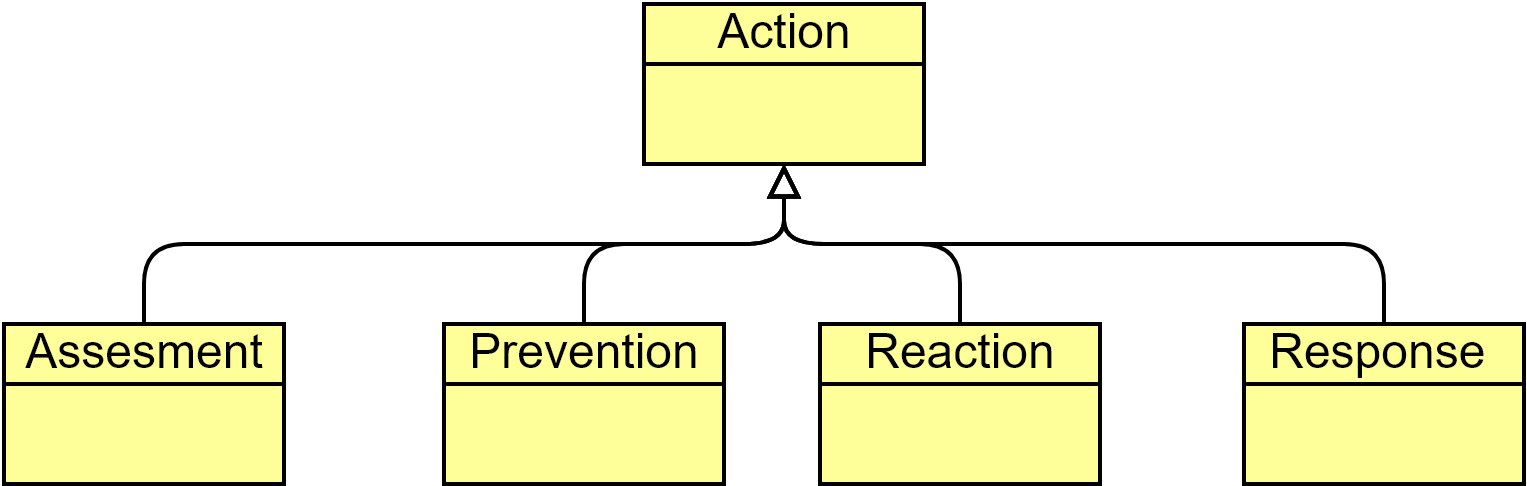
\includegraphics[width=4.36in,height=1.37in]{images/image6.png}
		\caption{Types of actions in a crisis}
		\label{fig:Types_of_actions_in_a_crisis}
	\end{Center}
\end{figure}
%%%%%%%%%%%%%%%%%%%% Figure/Image No: 1 Ends here %%%%%%%%%%%%%%%%%%%%
\end{Center}

``Action''  is a broad term covering all sorts of activities. Under it are depicted four classes of actions: the first two (on the left side of the diagram) are notably occurring before the crisis event happens. The other two (on the right side of the chart) apply to the aftermath. The depiction of the types of actions ordered sequentially along the temporal axis is depicted in Figure \ref{fig:Phases_in_crisis_management} where the crisis event takes a central place. 

\begin{Center}
%%%%%%%%%%%%%%%%%%%% Figure/Image No: 2 starts here %%%%%%%%%%%%%%%%%%%%

\begin{figure}[H]
	\begin{Center}
		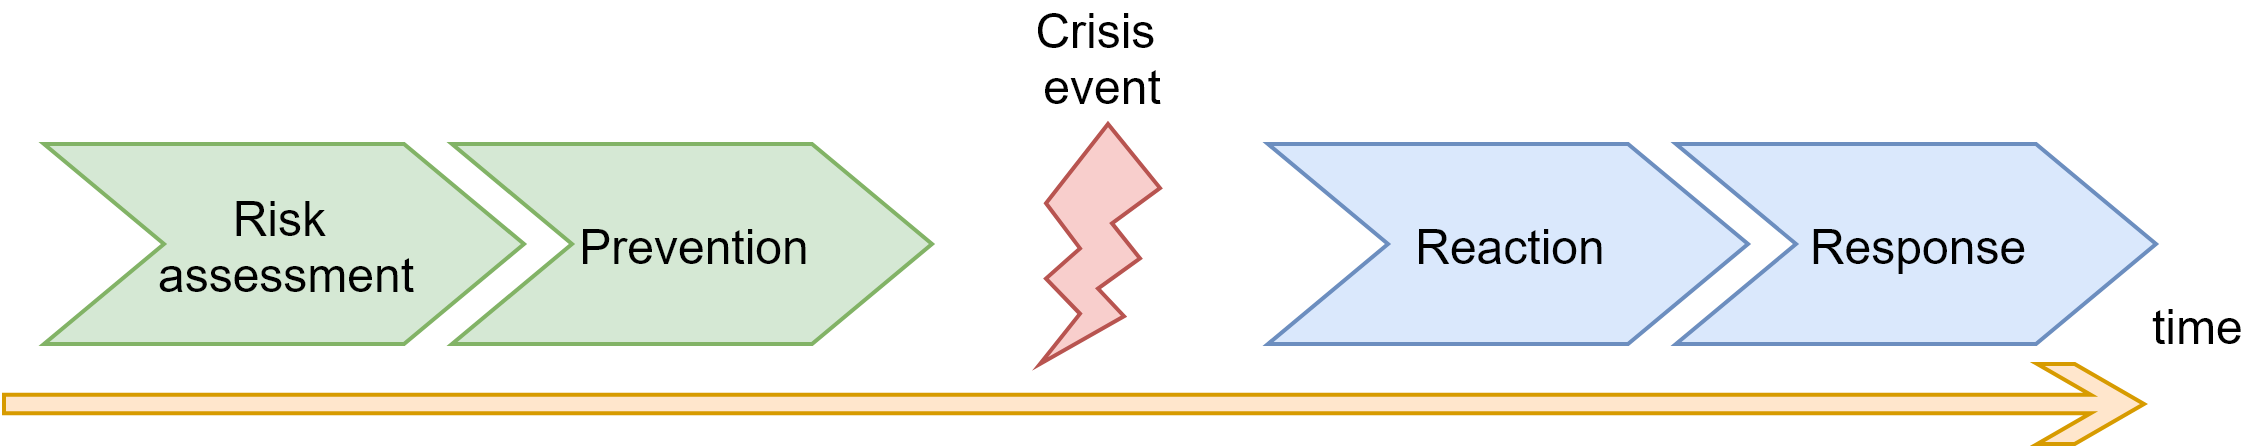
\includegraphics[width=\textwidth]{images/image4.png}
		\caption{Phases in crisis management}
		\label{fig:Phases_in_crisis_management}
	\end{Center}
\end{figure}
%%%%%%%%%%%%%%%%%%%% Figure/Image No: 2 Ends here %%%%%%%%%%%%%%%%%%%%
\end{Center}

The \textit{risk assessment} actions deal with risk identification, estimation of probability for each risk factor to occur. Also, at this stage is investigated the impact from the environmental, economic, social and public health perspectives, including who is impacted, how, and to what degree. 

The \textit{prevention} actions focus on what could be done to mitigate and alleviate the crisis impact in case it occurs. 

The \textit{crisis event} (or period) leads to an unstable and dangerous situation affecting an individual, group, or all of society. 

The \textit{reaction} actions deal with immediate mitigation while the \textit{responses} with medium to long-term mitigate the crisis consequences. These two action types: responses and reactions, which we collectively call \textit{measures}, and in our case \textit{measures to the COVID-19 crisis}, are the primary focus of the dataset. So, next, we define them in this context specifically. 

The \textit{COVID-19 reaction} is what an organisation plans to do to minimise the impact of the pandemics, such as including extra protective equipment for health workers, procurement of additional medical equipment, the introduction of social distancing, more rigorous border controls or their temporary closure. The reactions are actions related to the pandemic poses' health threats: ``a virus makes people sick, and something must be done about that'' . In addition to the pandemic consequences, the reactions have economic and social effects that can be directly observed or indirectly deduced. And so the reaction of the authorities to the virus affects the people too: consider, for example, the social distancing or the lockdown measures. We can say that the reactions are, in fact, to the health threat and that the main topics are anything related to health, pandemics, virus, infection etc. 

The \textit{COVID-19 responses} are measures set in place to compensate for the economic and social consequences of the pandemic crisis and diminish the effects of the authorities' reactions to the threat. Therefore the temporal horizon of the responses is much longer, and the topics they deal with are much broader and challenging to pinpoint. They could be anything related to social, economic, welfare, child care, telework, income support, increase in social protection and many other topics. 

Now, that the dataset domain is set to the COVID-19 reaction and response measures, with a predominant preference for the COVID-19 responses, we describe other criteria and provide some of our assumptions.  

\section{Criteria and assumptions about the data}
\label{sec:criteria}

\begin{itemize}
	\item Identify references to sources of data from discussions with the stakeholders and investigate them. From the selected ones collect text and metadata describing and classifying responses and reactions to the COVID-19 crisis. 
	\item To the extent possible, distinguish between reaction and response measures (as explained in Section \ref{sec:domain-delimitation}) because of the current project scope. 
	\item We assume that the official documents are a reliable source of measure descriptions.
	\item The primary focus is on collecting official texts of various registers (administrative, journalistic, legal, etc.) to enable further exercises to train machine learning models that can identify and distinguish a COVID-19 measure from other texts and, if possible, differences between the reactions and responses.
	\item Selecting the texts with these properties leads to a relatively scarce set of available resources. Therefore no (data) sampling was considered or any tests for the (data) balancing. Mainly we aimed at covering selected initial sources given the apparent degree of (data) representativeness to the semantic domain, which remains to be tested and analysed.
	\item We could identify two text registers (or genres) in the available sources, which is a valuable distinction in the further analysis. First is the journalistic or reportage style of language, which summarises and describes COVID-19 measures. Second is the legal style of language that characterises the source texts from where COVID-19 actions summaries are extracted. Possibly more genres could be identified in a detailed analysis. 
	\item Geographically, we select texts produced in the European Union, both at the EU level, by the institutions and at the member state level, by the national governments. 
	\item We select texts written in English as a first step and as an established limit to the scope, and later, in future work, this can be extended to texts written in the official EU 24 languages.
	\item We consider only texts issued after the beginning of 2020 when the COVID-19 pandemic started.

	\item A basic assumption is that Policy Watch Database (PWDB) is a suitable set of summarised descriptions of what a COVID-19 measure looks like. They cover broader economic and social issues in the area of working and living conditions and intentionally exclude COVID-19 reactions, which focus on public health-related issues. PWDB is a starting point and a pillar in developing this project. 
\end{itemize}

\section{Established data scope: how much is enough?}

Following an investigation and a series of discussions with the project stakeholders, it was decided to set the initial scope to collect data. This scope was set on pragmatic grounds with an awareness of possible extensions in future work.

This section presents the four datasets extracted from another source and constitute the current project dataset, Euro-COVID-19. The detailed description for each dataset is provided in a dedicated section below. Below is an outline of these datasets, along with their subcomponents. Note that the subcomponents are noteworthy at the level of this document to facilitate a deeper understanding of the data, but the dataset distributions merge them into usable wholes. We also provide a codified identifier for each dataset to allow for precise referencing.

\begin{itemize}
	\item \textbf{ds\_pwdb:} Policy Watch Dataset 
        \begin{itemize}
        	\item \textbf{what:} the content published on Eurofound website\footnote{ \href{https://www.eurofound.europa.eu/data/covid-19-eu-policywatch}{COVID-19 EU Policy Watch}}, that is enriched with content crawled from the referenced sources.
        	\item \textbf{why:} because it comprises a collection of manually authored documents summarising the COVID-19 response measures by the member states.
        \end{itemize}
	\item \textbf{ds\_eu\_cellar:} EU Cellar COVID-19 Dataset 
        \begin{itemize}
        	\item \textbf{what:} the EurLex\footnote{ \href{https://eur-lex.europa.eu/homepage.html}{EurLex: the portal to access European Union law} } documents fetched from Cellar\footnote{ \href{https://op.europa.eu/en/publication-detail/-/publication/50ecce27-857e-11e8-ac6a-01aa75ed71a1}{The semantic repository of the Publications Office} } marked with a special ``COVID-19'' tag. And, in addition, Cellar documents about selected EuroVoc\footnote{ \href{https://op.europa.eu/en/web/eu-vocabularies/dataset/-/resource?uri=http://publications.europa.eu/resource/dataset/eurovoc}{EuroVoc: The EU's Multilingual Thesaurus} } concepts (tightly related to COVID-19) dated after the 1st of January 2020.
        	\item \textbf{why:} because Cellar is the official EU semantic repository hosted by the Publications Office containing the official EU. documents. 
        \end{itemize}
	\item \textbf{ds\_eu\_timeline:} EU Action Timeline Dataset 
        \begin{itemize}
        	\item \textbf{what:} documents crawled from the EU action timeline website\footnote{ \href{https://ec.europa.eu/info/live-work-travel-eu/coronavirus-response/timeline-eu-action_en}{Timeline of EU action} }; and documents from the European Commission Press corner\footnote{ \href{https://ec.europa.eu/commission/presscorner/home/en}{Press material from the Commission Spokesperson's Service} } crawled by searching for selected EuroVoc concepts dated after 1st of January 2020.
        	\item \textbf{why:} because it comprises a curated list of official press releases on measures taken by the European Commission (the EU doer).
        \end{itemize}
	\item \textbf{ds\_ireland\_timeline:} Ireland COVID-19 Timeline Dataset
        \begin{itemize}
        	\item \textbf{what:} documents crawled from the Irish Government press corner by searching for pre-selected EuroVoc concepts dated after 1st of January 2020. 
        	\item \textbf{why:} it contains English language texts and constitutes an alternative source of (one) MS measures, which can be used to compare how ds\_pwdb covers a country. 
        \end{itemize}
\end{itemize}

\enlargethispage{1em}

The datasets listed above differ in terms of their internal structure and in terms of the content they cover. Each dataset will be presented in the sections below. A summary of the dataset content classification is provided in  Table \ref{tab:Classification of the dataset content}.

%%%%%%%%%%%%%%%%%%%% Table No: 2 starts here %%%%%%%%%%%%%%%%%%%%
\begin{table}[H]
 			\centering
\begin{tabular}{p{1.25in}p{1.25in}p{1.25in}p{1.25in}}
\hline
%row no:1
\multicolumn{1}{|p{1.25in}}{\Centering \textbf{@en}} & 
\multicolumn{1}{|p{1.25in}}{\Centering \textbf{EU}} & 
\multicolumn{1}{|p{1.25in}}{\Centering \textbf{MS (collectively)}} & 
\multicolumn{1}{|p{1.25in}|}{\Centering \textbf{MS (individual)}} \\
\hhline{----}
%row no:2
\multicolumn{1}{|p{1.25in}}{\Centering Journalistic text} & 
\multicolumn{1}{|p{1.25in}}{\Centering EU actions timeline} & 
\multicolumn{1}{|p{1.25in}}{\Centering Policy Watch DB} & 
\multicolumn{1}{|p{1.25in}|}{\Centering Ireland timeline} \\
\hhline{----}
%row no:3
\multicolumn{1}{|p{1.25in}}{\Centering Legal text} & 
\multicolumn{1}{|p{1.25in}}{\Centering EU Cellar COVID-19} & 
\multicolumn{1}{|p{1.25in}}{\Centering -} & 
\multicolumn{1}{|p{1.25in}|}{\Centering -} \\
\hhline{----}

\end{tabular}\caption{Classification of the dataset content}
\label{tab:Classification of the dataset content}
 \end{table}
\vspace{-1em}
%%%%%%%%%%%%%%%%%%% Table No: 2 ends here %%%%%%%%%%%%%%%%%%%%

In terms of content coverage, we distinguish datasets that cover: the EU measures, the MS measures for all EU states in a single collection, the MS measures segregated for each country. 

In terms of language register\footnote{Register (in Sociolinguistics) is a variety of language used for a particular purpose or in a particular communicative situation. This term is remotely synonym to text type, style and genre.} two major ones are identified that characterise existent texts: (a) \textit{Journalistic or reportage text register} and (b) \textit{formal administrative and legal text register}. The aim here is not to describe these registers but merely identify them as making such a distinction may be of significant relevance in the data analysis phase. 

Datasets pertaining to the journalistic(reportage) text register are

\begin{itemize}
	\item Policy Watch Database 
	\item EU action timeline

	\item Ireland action timeline
\end{itemize}

In the formal administrative and legal text register fall the following datasets

\begin{itemize}
	\item EU Cellar COVID-19 
\end{itemize}

In the next section we proceed with describing the structure for each dataset and some of its peculiarities.

\section{Dataset description: what is inside? }

This section describes the datasets in terms of their structure, scope and manner in which the data have been collected. 

\subsection{Policy watch database (ds\_pwdb)}

Eurofound's COVID-19 EU PolicyWatch (PWDB)\footnote{ PWDB download page  } collates information on the responses of government and social partners to the crisis, as well as gathering examples of company practices aimed at mitigating the social and economic impacts. Data has been mainly provided by the Network of Eurofound Correspondents, with quality control carried out by Eurofound staff.

PWDB includes large-scale government measures and wider collective agreements, as well as regional and local initiatives and support measures for smaller groups of workers. As the situation is evolving, measures are newly implemented, changed or cancelled and replaced at rapid speed. It is planned to update the cases with information on the actual uptake of the main measures. Outside the scope of this database are public health measures, travel and movement restrictions and company-specific job losses. 

The original PWDB contains a rich set of attributes. Only a subset is considered relevant from the business perspective to the current project and is listed in the table below. The original structure is transformed into a simplified form for harmonisation with other datasets and easier usage. The data structure of the transformed core PWDB dataset (ds\_pwdb\_core) is described in Table \ref{tab:dspwdbcore}.

In column BF are provided references to the business features for each data attribute. However, it is not always possible to establish a reliable one to one mapping. Therefore, in some places, we use: the tilde sign ($\sim$) to signify an approximate relation, the plus sign to signify that more than one BF is included or represented by the data attribute.

%%%%%%%%%%%%%%%%%%%% Table No: 3 starts here %%%%%%%%%%%%%%%%%%%%
{
\setlength\extrarowheight{3pt}
\begin{longtable}{p{1.16in}p{3.48in}p{0.62in}}

\endfirsthead
\multicolumn{3}{c}{\textit{continued from previous page}}%\hline
\endhead
\multicolumn{3}{r}{\textit{continued on next page}} \\
\endfoot
\endlastfoot\hline
%row no:1
\multicolumn{1}{|p{1.16in}}{\textbf{Data attribute}} & 
\multicolumn{1}{|p{3.48in}}{\textbf{Description}} & 
\multicolumn{1}{|p{0.62in}|}{\textbf{BF}} \\
\hhline{---}
%row no:2
\multicolumn{1}{|p{1.16in}}{Category} & 
\multicolumn{1}{|p{3.48in}}{Nine\ high-level categories for grouping the COVID-19 measures  (proposed by the EuroFond team\footnote{ About Eurofound }).} & 
\multicolumn{1}{|p{0.62in}|}{BF2} \\
\hhline{---}
%row no:3
\multicolumn{1}{|p{1.16in}}{Subcategory} & 
\multicolumn{1}{|p{3.48in}}{Further categorisation into fine grained categories, under a parent category. The two level taxonomy is not documented here but can be recreated from the dataset. } & 
\multicolumn{1}{|p{0.62in}|}{BF2} \\
\hhline{---}
%row no:4
\multicolumn{1}{|p{1.16in}}{Target group (L1)} & 
\multicolumn{1}{|p{3.48in}}{The database provides target groups for each measure. Target groups are organised on two levels: L1 $\&$  L2. The L1 level broadly differentiates between \textit{workers, businesses} and \textit{citizens}.} & 
\multicolumn{1}{|p{0.62in}|}{BF8} \\
\hhline{---}
%row no:5
\multicolumn{1}{|p{1.16in}}{Target group (L2)} & 
\multicolumn{1}{|p{3.48in}}{The L2 level contains more fine grained distinctions containing 42 specific target groups distinctions in total, including for example: \par \begin{itemize}
	\item Workers: \href{https://static.Eurofound.europa.eu/COVID-19db/targetGroups/self-employed.html}{\textcolor[HTML]{1155CC}{\ul{Self-employed}}}, \href{https://static.Eurofound.europa.eu/COVID-19db/targetGroups/seasonal_workers.html}{\textcolor[HTML]{1155CC}{\ul{Seasonal workers}}}, \href{https://static.Eurofound.europa.eu/COVID-19db/targetGroups/platform_workers.html}{\textcolor[HTML]{1155CC}{\ul{Platform workers}}}, etc. \par 	\item Businesses: \href{https://static.Eurofound.europa.eu/COVID-19db/targetGroups/smes.html}{\textcolor[HTML]{1155CC}{\ul{SMEs}}}, \href{https://static.Eurofound.europa.eu/COVID-19db/targetGroups/start-ups.html}{\textcolor[HTML]{1155CC}{\ul{Start-ups}}}, \href{https://static.Eurofound.europa.eu/COVID-19db/targetGroups/larger_corporations.html}{\textcolor[HTML]{1155CC}{\ul{Larger corporations}}}, etc. \par 	\item Citizens: \href{https://static.Eurofound.europa.eu/COVID-19db/targetGroups/parents.html}{\textcolor[HTML]{1155CC}{\ul{Parents}}}, \href{https://static.Eurofound.europa.eu/COVID-19db/targetGroups/older_citizens.html}{\textcolor[HTML]{1155CC}{\ul{Older citizens}}}, \href{https://static.Eurofound.europa.eu/COVID-19db/targetGroups/migrants.html}{\textcolor[HTML]{1155CC}{\ul{Migrants}}}, etc.
\end{itemize}} & 
\multicolumn{1}{|p{0.62in}|}{BF8} \\
\hhline{---}
%row no:6
\multicolumn{1}{|p{1.16in}}{Country} & 
\multicolumn{1}{|p{3.48in}}{The country where the COVID-19 measure is adopted by the government and social partners.} & 
\multicolumn{1}{|p{0.62in}|}{BF5, BF1} \\
\hhline{---}
%row no:7
\multicolumn{1}{|p{1.16in}}{Involved actors} & 
\multicolumn{1}{|p{3.48in}}{Eurofound identified 757 legislations and other statutory regulations, 452 of which have been created entirely in the context of COVID-19. This section gives an overview of social partner's involvement in designing and implementing these measures.} & 
\multicolumn{1}{|p{0.62in}|}{$ \sim $  (BF1 + BF8)} \\
\hhline{---}
%row no:8
\multicolumn{1}{|p{1.16in}}{Funding} & 
\multicolumn{1}{|p{3.48in}}{The sources of financing the measure, if the measure involves financial expenditures. Some measures do not have fundings. } & 
\multicolumn{1}{|p{0.62in}|}{$ \sim $  BF6} \\
\hhline{---}
%row no:9
\multicolumn{1}{|p{1.16in}}{Type} & 
\multicolumn{1}{|p{3.48in}}{Classification of the document types from where the description of the measures originates. Six types of source documents are distinguished, including legislations, collective agreements, recommendations and company practices.} & 
\multicolumn{1}{|p{0.62in}|}{} \\
\hhline{---}
%row no:10
\multicolumn{1}{|p{1.16in}}{Start $\&$  End dates} & 
\multicolumn{1}{|p{3.48in}}{The time period when the measure is applied.} & 
\multicolumn{1}{|p{0.62in}|}{BF4} \\
\hhline{---}
%row no:11
\multicolumn{1}{|p{1.16in}}{Creation date} & 
\multicolumn{1}{|p{3.48in}}{When the measure entry was created in the database.} & 
\multicolumn{1}{|p{0.62in}|}{$ \sim $  BF3} \\
\hhline{---}
%row no:12
\multicolumn{1}{|p{1.16in}}{Update date} & 
\multicolumn{1}{|p{3.48in}}{When last changes were made to the measure entry description.} & 
\multicolumn{1}{|p{0.62in}|}{$ \sim $  BF3} \\
\hhline{---}
%row no:13
\multicolumn{1}{|p{1.16in}}{Background information} & 
\multicolumn{1}{|p{3.48in}}{A short text providing the context and background information useful to understand the measure description.} & 
\multicolumn{1}{|p{0.62in}|}{BF10} \\
\hhline{---}
%row no:14
\multicolumn{1}{|p{1.16in}}{Content of measure} & 
\multicolumn{1}{|p{3.48in}}{A short text representing the abstract or a concise description of the measure.} & 
\multicolumn{1}{|p{0.62in}|}{BF10} \\
\hhline{---}
%row no:15
\multicolumn{1}{|p{1.16in}}{Content updates} & 
\multicolumn{1}{|p{3.48in}}{Short updates to the content of the measure.} & 
\multicolumn{1}{|p{0.62in}|}{BF10} \\
\hhline{---}
%row no:16
\multicolumn{1}{|p{1.16in}}{Use of measure} & 
\multicolumn{1}{|p{3.48in}}{Information about the results and outcomes of executing/enacting the measure.} & 
\multicolumn{1}{|p{0.62in}|}{BF10} \\
\hhline{---}
%row no:17
\multicolumn{1}{|p{1.16in}}{Title} & 
\multicolumn{1}{|p{3.48in}}{A short text used to identify the measure, place it in context, and convey a minimal summary of its contents.} & 
\multicolumn{1}{|p{0.62in}|}{BF10} \\
\hhline{---}
\caption{The attribute structure for core PWDB dataset (ds\_pwdb\_core)}
\label{tab:dspwdbcore}
\end{longtable}}



%%%%%%%%%%%%%%%%%%%% Table No: 3 ends here %%%%%%%%%%%%%%%%%%%%

In the core dataset, a list of source references is provided. They represent links to the original documents elaborating on the contents of the measure. We proceeded with downloading, cleaning and injecting the content of the sources into the PWD dataset, this way extending it.  
An additional set of data attributes is provided in the extended version of the PWDB dataset, as is listed in  Table \ref{tab:dspwdbext)}.

%%%%%%%%%%%%%%%%%%%% Table No: 4 starts here %%%%%%%%%%%%%%%%%%%%
\begin{table}[H]
 			\centering
\begin{tabular}{p{1.04in}p{4.24in}p{0.39in}}
\hline
%row no:1
\multicolumn{1}{|p{1.04in}}{\textbf{Data attribute}} & 
\multicolumn{1}{|p{4.24in}}{\textbf{Description}} & 
\multicolumn{1}{|p{0.39in}|}{\textbf{BF}} \\
\hhline{---}
%row no:2
\multicolumn{1}{|p{1.04in}}{Source URL} & 
\multicolumn{1}{|p{4.24in}}{The measure descriptions are based on external sources referenced by URLs} & 
\multicolumn{1}{|p{0.39in}|}{} \\
\hhline{---}
%row no:3
\multicolumn{1}{|p{1.04in}}{Source content} & 
\multicolumn{1}{|p{4.24in}}{The content (in simple text) downloaded by accessing the document at the source URL.} & 
\multicolumn{1}{|p{0.39in}|}{BF10} \\
\hhline{---}
%row no:4
\multicolumn{1}{|p{1.04in}}{Source title} & 
\multicolumn{1}{|p{4.24in}}{The title of the source document, if possible to retrieve} & 
\multicolumn{1}{|p{0.39in}|}{BF10} \\
\hhline{---}
%row no:5
\multicolumn{1}{|p{1.04in}}{Source language} & 
\multicolumn{1}{|p{4.24in}}{The language of the source content is determined by a language identification system.} & 
\multicolumn{1}{|p{0.39in}|}{} \\
\hhline{---}

\end{tabular}
\caption{The additional set of attributes constituting the PWBD extension (ds\_pwdb\_ext)}
\label{tab:dspwdbext)}
\end{table}
%%%%%%%%%%%%%%%%%%%% Table No: 4 ends here %%%%%%%%%%%%%%%%%%%%

Finally, the core and the extended dataset variants are merged and provided as a unified PWDB dataset. 

\enlargethispage{1em}

\subsection{EU Cellar COVID-19 dataset (ds\_eu\_cellar)}

The Cellar is the semantic repository of the Publications Office. It stores essential legal documents, general publications and other vital EU level documents. We query this repository to construct the EU level COVID-19 datasets containing the document content and the associated metadata. 

In the context of the current exercise, we distinguish the core and the extended datasets variants, which are results of querying Cellar with two different SPARQL queries.

The core dataset is the result of querying for documents (called works) that are annotated with a special ``COVID-19''  tag in the Cellar repository. The tagging is performed manually by the EurLex team and its contractors. This tag marks documents that have been identified as dealing directly with issues of the COVID-19 pandemic. 

The extended dataset is also the result of querying for documents (called works) in Cellar, which are annotated with any of the pre-selected EuroVoc concepts. We have manually selected concepts from the EuroVoc thesaurus judging whether a concept is or is not relevant to the COVID-19 pandemics. The relevance criteria covers both: the reaction topics, those pertaining to the public health domain, and the response topics, those pertaining to broader social and economic domains (for domain delineation see Section \ref{sec:domain-delimitation} ). The list of selected EuroVoc concepts is provided in  Table \ref{tab:EuroVoc concepts considered highly relevant for COVID-19 document search}. 

%%%%%%%%%%%%%%%%%%%% Table No: 5 starts here %%%%%%%%%%%%%%%%%%%%
{
\setlength\extrarowheight{3pt}
\begin{longtable}{p{2.5in}p{2.96in}}

\endfirsthead
\multicolumn{2}{c}{\textit{continued from previous page}} %\hline
\endhead
\multicolumn{2}{r}{\textit{continued on next page}} \\
\endfoot
\endlastfoot\hline
%row no:1
\multicolumn{1}{|p{2.5in}}{\textbf{Concept URI}} & 
\multicolumn{1}{|p{2.96in}|}{\textbf{Concept preferred label}} \\
\hhline{--}
%row no:2
\multicolumn{1}{|p{2.5in}}{{\fontsize{10pt}{12.0pt}\selectfont http://eurovoc.europa.eu/1005}} & 
\multicolumn{1}{|p{2.96in}|}{{\fontsize{10pt}{12.0pt}\selectfont EU financing}} \\
\hhline{--}
%row no:3
\multicolumn{1}{|p{2.5in}}{{\fontsize{10pt}{12.0pt}\selectfont http://eurovoc.europa.eu/1439}} & 
\multicolumn{1}{|p{2.96in}|}{{\fontsize{10pt}{12.0pt}\selectfont innovation}} \\
\hhline{--}
%row no:4
\multicolumn{1}{|p{2.5in}}{{\fontsize{10pt}{12.0pt}\selectfont http://eurovoc.europa.eu/1633}} & 
\multicolumn{1}{|p{2.96in}|}{{\fontsize{10pt}{12.0pt}\selectfont free movement of persons}} \\
\hhline{--}
%row no:5
\multicolumn{1}{|p{2.5in}}{{\fontsize{10pt}{12.0pt}\selectfont http://eurovoc.europa.eu/1754}} & 
\multicolumn{1}{|p{2.96in}|}{{\fontsize{10pt}{12.0pt}\selectfont illness}} \\
\hhline{--}
%row no:6
\multicolumn{1}{|p{2.5in}}{{\fontsize{10pt}{12.0pt}\selectfont http://eurovoc.europa.eu/1756}} & 
\multicolumn{1}{|p{2.96in}|}{{\fontsize{10pt}{12.0pt}\selectfont respiratory disease}} \\
\hhline{--}
%row no:7
\multicolumn{1}{|p{2.5in}}{{\fontsize{10pt}{12.0pt}\selectfont http://eurovoc.europa.eu/1759}} & 
\multicolumn{1}{|p{2.96in}|}{{\fontsize{10pt}{12.0pt}\selectfont infectious disease}} \\
\hhline{--}
%row no:8
\multicolumn{1}{|p{2.5in}}{{\fontsize{10pt}{12.0pt}\selectfont http://eurovoc.europa.eu/1802}} & 
\multicolumn{1}{|p{2.96in}|}{{\fontsize{10pt}{12.0pt}\selectfont labour market}} \\
\hhline{--}
%row no:9
\multicolumn{1}{|p{2.5in}}{{\fontsize{10pt}{12.0pt}\selectfont http://eurovoc.europa.eu/1854}} & 
\multicolumn{1}{|p{2.96in}|}{{\fontsize{10pt}{12.0pt}\selectfont disease prevention}} \\
\hhline{--}
%row no:10
\multicolumn{1}{|p{2.5in}}{{\fontsize{10pt}{12.0pt}\selectfont http://eurovoc.europa.eu/192}} & 
\multicolumn{1}{|p{2.96in}|}{{\fontsize{10pt}{12.0pt}\selectfont health control}} \\
\hhline{--}
%row no:11
\multicolumn{1}{|p{2.5in}}{{\fontsize{10pt}{12.0pt}\selectfont http://eurovoc.europa.eu/2916}} & 
\multicolumn{1}{|p{2.96in}|}{{\fontsize{10pt}{12.0pt}\selectfont applied research}} \\
\hhline{--}
%row no:12
\multicolumn{1}{|p{2.5in}}{{\fontsize{10pt}{12.0pt}\selectfont http://eurovoc.europa.eu/2923}} & 
\multicolumn{1}{|p{2.96in}|}{{\fontsize{10pt}{12.0pt}\selectfont medical research}} \\
\hhline{--}
%row no:13
\multicolumn{1}{|p{2.5in}}{{\fontsize{10pt}{12.0pt}\selectfont http://eurovoc.europa.eu/3730}} & 
\multicolumn{1}{|p{2.96in}|}{{\fontsize{10pt}{12.0pt}\selectfont health risk}} \\
\hhline{--}
%row no:14
\multicolumn{1}{|p{2.5in}}{{\fontsize{10pt}{12.0pt}\selectfont http://eurovoc.europa.eu/3885}} & 
\multicolumn{1}{|p{2.96in}|}{{\fontsize{10pt}{12.0pt}\selectfont public health}} \\
\hhline{--}
%row no:15
\multicolumn{1}{|p{2.5in}}{{\fontsize{10pt}{12.0pt}\selectfont http://eurovoc.europa.eu/4470}} & 
\multicolumn{1}{|p{2.96in}|}{{\fontsize{10pt}{12.0pt}\selectfont tourism}} \\
\hhline{--}
%row no:16
\multicolumn{1}{|p{2.5in}}{{\fontsize{10pt}{12.0pt}\selectfont http://eurovoc.europa.eu/4505}} & 
\multicolumn{1}{|p{2.96in}|}{{\fontsize{10pt}{12.0pt}\selectfont air transport}} \\
\hhline{--}
%row no:17
\multicolumn{1}{|p{2.5in}}{{\fontsize{10pt}{12.0pt}\selectfont http://eurovoc.europa.eu/5237}} & 
\multicolumn{1}{|p{2.96in}|}{{\fontsize{10pt}{12.0pt}\selectfont research and development}} \\
\hhline{--}
%row no:18
\multicolumn{1}{|p{2.5in}}{{\fontsize{10pt}{12.0pt}\selectfont http://eurovoc.europa.eu/835}} & 
\multicolumn{1}{|p{2.96in}|}{{\fontsize{10pt}{12.0pt}\selectfont aid to undertakings}} \\
\hhline{--}
%row no:19
\multicolumn{1}{|p{2.5in}}{{\fontsize{10pt}{12.0pt}\selectfont http://eurovoc.europa.eu/1280}} & 
\multicolumn{1}{|p{2.96in}|}{{\fontsize{10pt}{12.0pt}\selectfont occupational health}} \\
\hhline{--}
%row no:20
\multicolumn{1}{|p{2.5in}}{{\fontsize{10pt}{12.0pt}\selectfont http://eurovoc.europa.eu/1634}} & 
\multicolumn{1}{|p{2.96in}|}{{\fontsize{10pt}{12.0pt}\selectfont free movement of workers}} \\
\hhline{--}
%row no:21
\multicolumn{1}{|p{2.5in}}{{\fontsize{10pt}{12.0pt}\selectfont http://eurovoc.europa.eu/2062}} & 
\multicolumn{1}{|p{2.96in}|}{{\fontsize{10pt}{12.0pt}\selectfont standard of living}} \\
\hhline{--}
%row no:22
\multicolumn{1}{|p{2.5in}}{{\fontsize{10pt}{12.0pt}\selectfont http://eurovoc.europa.eu/2479}} & 
\multicolumn{1}{|p{2.96in}|}{{\fontsize{10pt}{12.0pt}\selectfont health policy}} \\
\hhline{--}
%row no:23
\multicolumn{1}{|p{2.5in}}{{\fontsize{10pt}{12.0pt}\selectfont http://eurovoc.europa.eu/5891}} & 
\multicolumn{1}{|p{2.96in}|}{{\fontsize{10pt}{12.0pt}\selectfont public awareness campaign}} \\
\hhline{--}
%row no:24
\multicolumn{1}{|p{2.5in}}{{\fontsize{10pt}{12.0pt}\selectfont http://eurovoc.europa.eu/82}} & 
\multicolumn{1}{|p{2.96in}|}{{\fontsize{10pt}{12.0pt}\selectfont working conditions}} \\
\hhline{--}
%row no:25
\multicolumn{1}{|p{2.5in}}{{\fontsize{10pt}{12.0pt}\selectfont http://eurovoc.europa.eu/2473}} & 
\multicolumn{1}{|p{2.96in}|}{{\fontsize{10pt}{12.0pt}\selectfont communications policy}} \\
\hhline{--}
%row no:26
\multicolumn{1}{|p{2.5in}}{{\fontsize{10pt}{12.0pt}\selectfont http://eurovoc.europa.eu/3086}} & 
\multicolumn{1}{|p{2.96in}|}{{\fontsize{10pt}{12.0pt}\selectfont economic consequence}} \\
\hhline{--}
%row no:27
\multicolumn{1}{|p{2.5in}}{{\fontsize{10pt}{12.0pt}\selectfont http://eurovoc.europa.eu/4636}} & 
\multicolumn{1}{|p{2.96in}|}{{\fontsize{10pt}{12.0pt}\selectfont vaccination}} \\
\hhline{--}
%row no:28
\multicolumn{1}{|p{2.5in}}{{\fontsize{10pt}{12.0pt}\selectfont http://eurovoc.europa.eu/5992}} & 
\multicolumn{1}{|p{2.96in}|}{{\fontsize{10pt}{12.0pt}\selectfont economic activity}} \\
\hhline{--}
%row no:29
\multicolumn{1}{|p{2.5in}}{{\fontsize{10pt}{12.0pt}\selectfont http://eurovoc.europa.eu/712}} & 
\multicolumn{1}{|p{2.96in}|}{{\fontsize{10pt}{12.0pt}\selectfont economic support}} \\
\hhline{--}
%row no:30
\multicolumn{1}{|p{2.5in}}{{\fontsize{10pt}{12.0pt}\selectfont http://eurovoc.europa.eu/826}} & 
\multicolumn{1}{|p{2.96in}|}{{\fontsize{10pt}{12.0pt}\selectfont aid to disadvantaged groups}} \\
\hhline{--}
%row no:31
\multicolumn{1}{|p{2.5in}}{{\fontsize{10pt}{12.0pt}\selectfont http://eurovoc.europa.eu/1596}} & 
\multicolumn{1}{|p{2.96in}|}{{\fontsize{10pt}{12.0pt}\selectfont health legislation}} \\
\hhline{--}
%row no:32
\multicolumn{1}{|p{2.5in}}{{\fontsize{10pt}{12.0pt}\selectfont http://eurovoc.europa.eu/2870}} & 
\multicolumn{1}{|p{2.96in}|}{{\fontsize{10pt}{12.0pt}\selectfont quality of life}} \\
\hhline{--}
%row no:33
\multicolumn{1}{|p{2.5in}}{{\fontsize{10pt}{12.0pt}\selectfont http://eurovoc.europa.eu/3956}} & 
\multicolumn{1}{|p{2.96in}|}{{\fontsize{10pt}{12.0pt}\selectfont social sciences}} \\
\hhline{--}
%row no:34
\multicolumn{1}{|p{2.5in}}{{\fontsize{10pt}{12.0pt}\selectfont http://eurovoc.europa.eu/899}} & 
\multicolumn{1}{|p{2.96in}|}{{\fontsize{10pt}{12.0pt}\selectfont economic aid}} \\
\hhline{--}
%row no:35
\multicolumn{1}{|p{2.5in}}{{\fontsize{10pt}{12.0pt}\selectfont http://eurovoc.europa.eu/7983}} & 
\multicolumn{1}{|p{2.96in}|}{{\fontsize{10pt}{12.0pt}\selectfont European Centre for Disease Prevention and Control}} \\
\hhline{--}
%row no:36
\multicolumn{1}{|p{2.5in}}{{\fontsize{10pt}{12.0pt}\selectfont http://eurovoc.europa.eu/83}} & 
\multicolumn{1}{|p{2.96in}|}{{\fontsize{10pt}{12.0pt}\selectfont living conditions}} \\
\hhline{--}
%row no:37
\multicolumn{1}{|p{2.5in}}{{\fontsize{10pt}{12.0pt}\selectfont http://eurovoc.europa.eu/85}} & 
\multicolumn{1}{|p{2.96in}|}{{\fontsize{10pt}{12.0pt}\selectfont social situation}} \\
\hhline{--}
%row no:38
\multicolumn{1}{|p{2.5in}}{{\fontsize{10pt}{12.0pt}\selectfont http://eurovoc.europa.eu/5764}} & 
\multicolumn{1}{|p{2.96in}|}{{\fontsize{10pt}{12.0pt}\selectfont organisation of health care}} \\
\hhline{--}
%row no:39
\multicolumn{1}{|p{2.5in}}{{\fontsize{10pt}{12.0pt}\selectfont http://eurovoc.europa.eu/3552}} & 
\multicolumn{1}{|p{2.96in}|}{{\fontsize{10pt}{12.0pt}\selectfont teleworking}} \\
\hhline{--}
%row no:40
\multicolumn{1}{|p{2.5in}}{{\fontsize{10pt}{12.0pt}\selectfont http://eurovoc.europa.eu/1742}} & 
\multicolumn{1}{|p{2.96in}|}{{\fontsize{10pt}{12.0pt}\selectfont job preservation}} \\
\hhline{--}
%row no:41
\multicolumn{1}{|p{2.5in}}{{\fontsize{10pt}{12.0pt}\selectfont http://eurovoc.europa.eu/886}} & 
\multicolumn{1}{|p{2.96in}|}{{\fontsize{10pt}{12.0pt}\selectfont state of emergency}} \\
\hhline{--}
%row no:42
\multicolumn{1}{|p{2.5in}}{{\fontsize{10pt}{12.0pt}\selectfont http://eurovoc.europa.eu/1926}} & 
\multicolumn{1}{|p{2.96in}|}{{\fontsize{10pt}{12.0pt}\selectfont working environment}} \\
\hhline{--}
%row no:43
\multicolumn{1}{|p{2.5in}}{{\fontsize{10pt}{12.0pt}\selectfont http://eurovoc.europa.eu/4116}} & 
\multicolumn{1}{|p{2.96in}|}{{\fontsize{10pt}{12.0pt}\selectfont health service}} \\
\hhline{--}
%row no:44
\multicolumn{1}{|p{2.5in}}{{\fontsize{10pt}{12.0pt}\selectfont http://eurovoc.europa.eu/5612}} & 
\multicolumn{1}{|p{2.96in}|}{{\fontsize{10pt}{12.0pt}\selectfont protective equipment}} \\
\hhline{--}
%row no:45
\multicolumn{1}{|p{2.5in}}{{\fontsize{10pt}{12.0pt}\selectfont http://eurovoc.europa.eu/837}} & 
\multicolumn{1}{|p{2.96in}|}{{\fontsize{10pt}{12.0pt}\selectfont epidemic}} \\
\hhline{--}
%row no:46
\multicolumn{1}{|p{2.5in}}{{\fontsize{10pt}{12.0pt}\selectfont http://eurovoc.europa.eu/2270}} & 
\multicolumn{1}{|p{2.96in}|}{{\fontsize{10pt}{12.0pt}\selectfont social participation}} \\
\hhline{--}
%row no:47
\multicolumn{1}{|p{2.5in}}{{\fontsize{10pt}{12.0pt}\selectfont http://eurovoc.europa.eu/838}} & 
\multicolumn{1}{|p{2.96in}|}{{\fontsize{10pt}{12.0pt}\selectfont epidemiology}} \\
\hhline{--}
%row no:48
\multicolumn{1}{|p{2.5in}}{{\fontsize{10pt}{12.0pt}\selectfont http://eurovoc.europa.eu/2793}} & 
\multicolumn{1}{|p{2.96in}|}{{\fontsize{10pt}{12.0pt}\selectfont aid programme}} \\
\hhline{--}
%row no:49
\multicolumn{1}{|p{2.5in}}{{\fontsize{10pt}{12.0pt}\selectfont http://eurovoc.europa.eu/3588}} & 
\multicolumn{1}{|p{2.96in}|}{{\fontsize{10pt}{12.0pt}\selectfont restriction of liberty}} \\
\hhline{--}
%row no:50
\multicolumn{1}{|p{2.5in}}{{\fontsize{10pt}{12.0pt}\selectfont http://eurovoc.europa.eu/6781}} & 
\multicolumn{1}{|p{2.96in}|}{{\fontsize{10pt}{12.0pt}\selectfont basic needs}} \\
\hhline{--}
%row no:51
\multicolumn{1}{|p{2.5in}}{{\fontsize{10pt}{12.0pt}\selectfont http://eurovoc.europa.eu/3371}} & 
\multicolumn{1}{|p{2.96in}|}{{\fontsize{10pt}{12.0pt}\selectfont public hygiene}} \\
\hhline{--}
%row no:52
\multicolumn{1}{|p{2.5in}}{{\fontsize{10pt}{12.0pt}\selectfont http://eurovoc.europa.eu/2013}} & 
\multicolumn{1}{|p{2.96in}|}{{\fontsize{10pt}{12.0pt}\selectfont mass media}} \\
\hhline{--}
%row no:53
\multicolumn{1}{|p{2.5in}}{{\fontsize{10pt}{12.0pt}\selectfont http://eurovoc.europa.eu/7131}} & 
\multicolumn{1}{|p{2.96in}|}{{\fontsize{10pt}{12.0pt}\selectfont social impact}} \\
\hhline{--}
%row no:54
\multicolumn{1}{|p{2.5in}}{{\fontsize{10pt}{12.0pt}\selectfont http://eurovoc.europa.eu/3906}} & 
\multicolumn{1}{|p{2.96in}|}{{\fontsize{10pt}{12.0pt}\selectfont freedom of movement}} \\
\hhline{--}
%row no:55
\multicolumn{1}{|p{2.5in}}{{\fontsize{10pt}{12.0pt}\selectfont http://eurovoc.europa.eu/3370}} & 
\multicolumn{1}{|p{2.96in}|}{{\fontsize{10pt}{12.0pt}\selectfont patient rights}} \\
\hhline{--}
%row no:56
\multicolumn{1}{|p{2.5in}}{{\fontsize{10pt}{12.0pt}\selectfont http://eurovoc.europa.eu/4881}} & 
\multicolumn{1}{|p{2.96in}|}{{\fontsize{10pt}{12.0pt}\selectfont social well-being}} \\
\hhline{--}
%row no:57
\multicolumn{1}{|p{2.5in}}{{\fontsize{10pt}{12.0pt}\selectfont http://eurovoc.europa.eu/86}} & 
\multicolumn{1}{|p{2.96in}|}{{\fontsize{10pt}{12.0pt}\selectfont socioeconomic conditions}} \\
\hhline{--}
%row no:58
\multicolumn{1}{|p{2.5in}}{{\fontsize{10pt}{12.0pt}\selectfont http://eurovoc.europa.eu/1758}} & 
\multicolumn{1}{|p{2.96in}|}{{\fontsize{10pt}{12.0pt}\selectfont endemic disease}} \\
\hhline{--}
%row no:59
\multicolumn{1}{|p{2.5in}}{{\fontsize{10pt}{12.0pt}\selectfont http://eurovoc.europa.eu/779}} & 
\multicolumn{1}{|p{2.96in}|}{{\fontsize{10pt}{12.0pt}\selectfont distance learning}} \\
\hhline{--}
%row no:60
\multicolumn{1}{|p{2.5in}}{{\fontsize{10pt}{12.0pt}\selectfont http://eurovoc.europa.eu/6609}} & 
\multicolumn{1}{|p{2.96in}|}{{\fontsize{10pt}{12.0pt}\selectfont self-regulation}} \\
\hhline{--}
%row no:61
\multicolumn{1}{|p{2.5in}}{{\fontsize{10pt}{12.0pt}\selectfont http://eurovoc.europa.eu/6770}} & 
\multicolumn{1}{|p{2.96in}|}{{\fontsize{10pt}{12.0pt}\selectfont disinformation}} \\
\hhline{--}
%row no:62
\multicolumn{1}{|p{2.5in}}{{\fontsize{10pt}{12.0pt}\selectfont http://eurovoc.europa.eu/c\_324b44f1}} & 
\multicolumn{1}{|p{2.96in}|}{{\fontsize{10pt}{12.0pt}\selectfont social media}} \\
\hhline{--}
%row no:63
\multicolumn{1}{|p{2.5in}}{{\fontsize{10pt}{12.0pt}\selectfont http://eurovoc.europa.eu/c\_5b447e3a}} & 
\multicolumn{1}{|p{2.96in}|}{{\fontsize{10pt}{12.0pt}\selectfont crisis management}} \\
\hhline{--}
%row no:64
\multicolumn{1}{|p{2.5in}}{{\fontsize{10pt}{12.0pt}\selectfont http://eurovoc.europa.eu/c\_31da5694}} & 
\multicolumn{1}{|p{2.96in}|}{{\fontsize{10pt}{12.0pt}\selectfont e-Health}} \\
\hhline{--}
%row no:65
\multicolumn{1}{|p{2.5in}}{{\fontsize{10pt}{12.0pt}\selectfont http://eurovoc.europa.eu/c\_60d3928d}} & 
\multicolumn{1}{|p{2.96in}|}{{\fontsize{10pt}{12.0pt}\selectfont patient safety}} \\
\hhline{--}
%row no:66
\multicolumn{1}{|p{2.5in}}{{\fontsize{10pt}{12.0pt}\selectfont http://eurovoc.europa.eu/c\_9b88f778}} & 
\multicolumn{1}{|p{2.96in}|}{{\fontsize{10pt}{12.0pt}\selectfont hospital infection}} \\
\hhline{--}
%row no:67
\multicolumn{1}{|p{2.5in}}{{\fontsize{10pt}{12.0pt}\selectfont http://eurovoc.europa.eu/c\_ece0a719}} & 
\multicolumn{1}{|p{2.96in}|}{{\fontsize{10pt}{12.0pt}\selectfont viral disease}} \\
\hhline{--}
%row no:68
\multicolumn{1}{|p{2.5in}}{{\fontsize{10pt}{12.0pt}\selectfont http://eurovoc.europa.eu/c\_814bb9e4}} & 
\multicolumn{1}{|p{2.96in}|}{{\fontsize{10pt}{12.0pt}\selectfont coronavirus disease}} \\
\hhline{--}
%row no:69
\multicolumn{1}{|p{2.5in}}{{\fontsize{10pt}{12.0pt}\selectfont http://eurovoc.europa.eu/c\_abfaf2ea}} & 
\multicolumn{1}{|p{2.96in}|}{{\fontsize{10pt}{12.0pt}\selectfont disease surveillance}} \\
\hhline{--}
\caption{EuroVoc concepts considered highly relevant for COVID-19 document search}\label{tab:EuroVoc concepts considered highly relevant for COVID-19 document search}
\end{longtable}}
%%%%%%%%%%%%%%%%%%%% Table No: 5 ends here %%%%%%%%%%%%%%%%%%%%

The result of querying Cellar in both cases (core and extended datasets) contains the same data attributes. The difference is in the retrieved documents. The structure of the eu\_cellar dataset is provided in  Table \ref{tab:The attribute structure for eu_cellar dataset}. 

%%%%%%%%%%%%%%%%%%%% Table No: 6 starts here %%%%%%%%%%%%%%%%%%%%
% \begin{table}[h]
%  			\centering
% \begin{tabular}{p{0.99in}p{3.86in}p{0.58in}}
% \hline
{
\setlength\extrarowheight{3pt}
\begin{longtable}{p{1.16in}p{3.48in}p{0.62in}}

\endfirsthead
\multicolumn{3}{c}{\textit{continued from previous page}}%\hline
\endhead
\multicolumn{3}{r}{\textit{continued on next page}} \\
\endfoot
\endlastfoot\hline
%row no:1
\multicolumn{1}{|p{0.99in}}{\textbf{Data attribute}} & 
\multicolumn{1}{|p{3.86in}}{\textbf{Description}} & 
\multicolumn{1}{|p{0.58in}|}{\textbf{BF}} \\
\hhline{---}
%row no:2
\multicolumn{1}{|p{0.99in}}{Work URI} & 
\multicolumn{1}{|p{3.86in}}{The URI, which is uniquely identifying the work.} & 
\multicolumn{1}{|p{0.58in}|}{} \\
\hhline{---}
%row no:3
\multicolumn{1}{|p{0.99in}}{CDM type} & 
\multicolumn{1}{|p{3.86in}}{The\ work type according to the Common Data Model ontology.  } & 
\multicolumn{1}{|p{0.58in}|}{} \\
\hhline{---}
%row no:4
\multicolumn{1}{|p{0.99in}}{Resource type} & 
\multicolumn{1}{|p{3.86in}}{The work type according to the OP classification used in the European inter-institutional exchange of legal documents. The resource types are organised in a classification scheme called Resource Type\footnote{ Resource Type authority table }. } & 
\multicolumn{1}{|p{0.58in}|}{} \\
\hhline{---}
%row no:5
\multicolumn{1}{|p{0.99in}}{EuroVoc concept} & 
\multicolumn{1}{|p{3.86in}}{The EuroVoc concept\footnote{ The EuroVoc thesaurus is represented as Concepts organised in ConceptSchemes following the Simple Knowledge Organisation System (SKOS). } used as a topic and classifier of the document content. The EuroVoc thesaurus is developed by the OP and used in the inter-institutional context. The concepts are organised as taxonomies from the broad to more narrow concepts. } & 
\multicolumn{1}{|p{0.58in}|}{BF2} \\
\hhline{---}
%row no:6
\multicolumn{1}{|p{0.99in}}{Subject matter} & 
\multicolumn{1}{|p{3.86in}}{The subject matter concept used as topic and classifier of the document content. The Subject Matter controlled vocabulary\footnote{ Subject Matter authority table } is developed by the OP and used in the inter-institutional context. The concepts are organised in a classification scheme called subject-matter, or FD\_070\footnote{ FD 070 ATTO table }. } & 
\multicolumn{1}{|p{0.58in}|}{BF2} \\
\hhline{---}
%row no:7
\multicolumn{1}{|p{0.99in}}{Directory code} & 
\multicolumn{1}{|p{3.86in}}{The directory code concept used to organise the legal documents in the EurLEx website. The concepts are organised in a classification scheme called FD\_555\footnote{ FD 555 ATTO table }.} & 
\multicolumn{1}{|p{0.58in}|}{$ \sim $  BF2} \\
\hhline{---}
%row no:8
\multicolumn{1}{|p{0.99in}}{Author} & 
\multicolumn{1}{|p{3.86in}}{The authors of the legal document. The identifier of the authors provided here is from the controlled list called Corporate Body\footnote{ Corporate body authority table }.} & 
\multicolumn{1}{|p{0.58in}|}{BF1} \\
\hhline{---}
%row no:9
\multicolumn{1}{|p{0.99in}}{Date document} & 
\multicolumn{1}{|p{3.86in}}{The date document was issued, entered into force, signed or other date relevant for the document legality.} & 
\multicolumn{1}{|p{0.58in}|}{BF3} \\
\hhline{---}
%row no:10
\multicolumn{1}{|p{0.99in}}{Content} & 
\multicolumn{1}{|p{3.86in}}{The actual content of the legal document, reduced to simple unstructured text.} & 
\multicolumn{1}{|p{0.58in}|}{BF10} \\
\hhline{---}
%row no:11
\multicolumn{1}{|p{0.99in}}{Title} & 
\multicolumn{1}{|p{3.86in}}{The document tile.} & 
\multicolumn{1}{|p{0.58in}|}{BF10} \\
\hhline{---}

% \end{tabular}
\caption{The attribute structure for eu\_cellar dataset}
\label{tab:The attribute structure for eu_cellar dataset}
%  \end{table}
\end{longtable}}
%%%%%%%%%%%%%%%%%%%% Table No: 6 ends here %%%%%%%%%%%%%%%%%%%%

Finally, the core and the extended dataset variants are merged and provided as a unified EU Cellar COVID-19 dataset. 

\subsection{EU action timeline dataset (ds\_eu\_timeline)}

The European Commission (EC) is coordinating a common European response to the coronavirus outbreak. EC is taking resolute action to reinforce our public health sectors and mitigate the socio-economic impact in the European Union. EC is mobilising means to help the Member States coordinate their national responses and provide objective information about the spread of the virus and practical efforts to contain it. 

The timeline of EU actions\footnote{ EU actions timeline website } during the COVID-19 pandemics is a website published by the EC with the most important COVID-19 responses. From 1104 actions (counted on 19/04/2021) published in the press corner only 171 were mentioned on the EU action timeline. So the timeline constitutes a refinement of the noteworthy and an aggregation of the EU actions. 

We crawl this website, and its content is automatically organised using the attributes listed in  Table \ref{tab:dseutimeline}. Unfortunately, only a very limited set of metadata can be identified in the crawled content: title, abstract, date of publication, and the actual content. And we know that the more metadata about a document, the better it is to answer some of the questions mentioned in the project goals section.

Following a discussion with the representatives of Directorate-General for Communication (DG COMM)\footnote{ The Directorate-General for Communication is the Commission department responsible for explaining EU policies to outside audiences. }, we identified a way to recover the possible topics using the name(s) of the authors for each article. This is possible because each author (spokesperson or press officer) is responsible for one or a few topics. These topics are assigned to each press contact who is on the spokesperson's service page\footnote{ Press contacts – Spokesperson's Service - list of possible article authors each covering one or few topics.}. 

What we did was to first extract and structure the information about each person and the topics he/she covers. Then we extended the original crawler to take into consideration this mapping between the person name and the topics. A new data attribute is created for each article containing the array of possible topics that characterise the article. 

Note that the list shall not be read as conjunction, that is: the article is about all of the topics provided; but as a disjunction, which means: the article is about one of the provided topics. 

%%%%%%%%%%%%%%%%%%%% Table No: 7 starts here %%%%%%%%%%%%%%%%%%%%
% \begin{table}[h]
%  			\centering
% \begin{tabular}{p{0.96in}p{3.87in}p{0.5in}}
% \hline
{
\setlength\extrarowheight{3pt}
\begin{longtable}{p{1.16in}p{3.48in}p{0.62in}}

\endfirsthead
\multicolumn{3}{c}{\textit{continued from previous page}}%\hline
\endhead
\multicolumn{3}{r}{\textit{continued on next page}} \\
\endfoot
\endlastfoot\hline

%row no:1
\multicolumn{1}{|p{0.96in}}{\textbf{Data attribute}} & 
\multicolumn{1}{|p{3.87in}}{\textbf{Description}} & 
\multicolumn{1}{|p{0.5in}|}{\textbf{BF}} \\
\hhline{---}
%row no:2
\multicolumn{1}{|p{0.96in}}{Abstract} & 
\multicolumn{1}{|p{3.87in}}{A short summary of the article, an abstract.} & 
\multicolumn{1}{|p{0.5in}|}{$ \sim $  BF3} \\
\hhline{---}
%row no:3
\multicolumn{1}{|p{0.96in}}{Content} & 
\multicolumn{1}{|p{3.87in}}{An extended description of the action as a press release article. } & 
\multicolumn{1}{|p{0.5in}|}{BF10} \\
\hhline{---}
%row no:4
\multicolumn{1}{|p{0.96in}}{Date} & 
\multicolumn{1}{|p{3.87in}}{The date when the press release was published} & 
\multicolumn{1}{|p{0.5in}|}{BF10} \\
\hhline{---}
%row no:5
\multicolumn{1}{|p{0.96in}}{Title} & 
\multicolumn{1}{|p{3.87in}}{The title of the press release article. } & 
\multicolumn{1}{|p{0.5in}|}{$ \sim $  BF10} \\
\hhline{---}
%row no:6
\multicolumn{1}{|p{0.96in}}{Topic} & 
\multicolumn{1}{|p{3.87in}}{A list of possible topics that the article may be about, derived from the author's thematic responsibility.} & 
\multicolumn{1}{|p{0.5in}|}{BF2} \\
\hhline{---}

% \end{tabular}
\caption{The attribute structure for ds\_eu\_timeline}
\label{tab:dseutimeline}

%  \end{table}
\end{longtable}}
%%%%%%%%%%%%%%%%%%%% Table No: 7 ends here %%%%%%%%%%%%%%%%%%%%

\subsection{Ireland COVID-19 timeline dataset}

Ireland was selected as a tryout member state country for which a COVID-19 timeline shall be created similar to the EU action timeline. It was selected because it is the only member state country (UK having just left the EU) that publishes official documents and press releases in English. 

An investigation was conducted searching for a comparable timeline summary of Ireland actions on COVID-19, and none was found. However, the official government website press corner, \href{http://www.gov.ie}{\textcolor[HTML]{1155CC}{\ul{www.gov.ie}}}, was identified as a good source of information. 

``gov.ie''  website is a central portal for government services and information. It combines the websites of Irish government departments and is a trusted source that makes interactions with the government more user-focused.

We decided to use the search service of this website and search for the same set of EuroVoc concepts that were used to retrieve COVID-19 relevant documents from Cellar. The search results are crawled and structured in a dataset using the set of data attributes listed in  Table \ref{tab:dsirelandtimeline}. 

The preferred label of each EuroVoc concept is used as a search term. For each EuroVoc concept, a new search is launched, and only articles that are more recent than the 1st of January 2020 are considered.

%%%%%%%%%%%%%%%%%%%% Table No: 8 starts here %%%%%%%%%%%%%%%%%%%%
% \begin{table}[h]
%  			\centering
% \begin{tabular}{p{1.21in}p{4.06in}p{0.35in}}
% \hline
{
\setlength\extrarowheight{3pt}
\begin{longtable}{p{1.16in}p{3.48in}p{0.62in}}

\endfirsthead
\multicolumn{3}{c}{\textit{continued from previous page}}%\hline
\endhead
\multicolumn{3}{r}{\textit{continued on next page}} \\
\endfoot
\endlastfoot\hline
%row no:1
\multicolumn{1}{|p{1.21in}}{\textbf{Data attribute}} & 
\multicolumn{1}{|p{4.06in}}{\textbf{Description}} & 
\multicolumn{1}{|p{0.35in}|}{\textbf{BF}} \\
\hhline{---}
%row no:2
\multicolumn{1}{|p{1.21in}}{Title} & 
\multicolumn{1}{|p{4.06in}}{The title of the press release article.} & 
\multicolumn{1}{|p{0.35in}|}{BF10} \\
\hhline{---}
%row no:3
\multicolumn{1}{|p{1.21in}}{Content} & 
\multicolumn{1}{|p{4.06in}}{The press release article in simple, clean unstructured text. } & 
\multicolumn{1}{|p{0.35in}|}{BF10} \\
\hhline{---}
%row no:4
\multicolumn{1}{|p{1.21in}}{Published date} & 
\multicolumn{1}{|p{4.06in}}{The date when the press release was published} & 
\multicolumn{1}{|p{0.35in}|}{BF3} \\
\hhline{---}
%row no:5
\multicolumn{1}{|p{1.21in}}{Update date} & 
\multicolumn{1}{|p{4.06in}}{The date when the article was updated.} & 
\multicolumn{1}{|p{0.35in}|}{$ \sim $ BF3} \\
\hhline{---}
%row no:6
\multicolumn{1}{|p{1.21in}}{Content links} & 
\multicolumn{1}{|p{4.06in}}{A list of links available in the text.} & 
\multicolumn{1}{|p{0.35in}|}{} \\
\hhline{---}
%row no:7
\multicolumn{1}{|p{1.21in}}{Campaigns links} & 
\multicolumn{1}{|p{4.06in}}{A list of links to the organised Campaigns} & 
\multicolumn{1}{|p{0.35in}|}{} \\
\hhline{---}
%row no:8
\multicolumn{1}{|p{1.21in}}{Department} & 
\multicolumn{1}{|p{4.06in}}{The government department that was authoring the article. } & 
\multicolumn{1}{|p{0.35in}|}{$ \sim $ BF1} \\
\hhline{---}
%row no:9
\multicolumn{1}{|p{1.21in}}{Policies links} & 
\multicolumn{1}{|p{4.06in}}{The list of links to the broad policy category under which the article is placed.} & 
\multicolumn{1}{|p{0.35in}|}{$ \sim $ BF2} \\
\hhline{---}
%row no:10
\multicolumn{1}{|p{1.21in}}{Keywords} & 
\multicolumn{1}{|p{4.06in}}{A list of keywords assigned by the article authors. } & 
\multicolumn{1}{|p{0.35in}|}{$ \sim $ BF2} \\
\hhline{---}
%row no:11
\multicolumn{1}{|p{1.21in}}{Page type} & 
\multicolumn{1}{|p{4.06in}}{The\ type of article is similar to the classification from the Resource Type authority table used for the ds\_eu\_cellar dataset. The possible types are the following: press release, speech, news, policy information,  reports, etc. } & 
\multicolumn{1}{|p{0.35in}|}{} \\
\hhline{---}

% \end{tabular}

\caption{The attribute structure for ds\_ireland\_timeline}
\label{tab:dsirelandtimeline}
% \end{table}

\end{longtable}}
%%%%%%%%%%%%%%%%%%%% Table No: 8 ends here %%%%%%%%%%%%%%%%%%%%

\section{Architectural overview}

This section presents the technology stack we employ and the design of the workflows for creating the datasets. An overview is depicted in the Figure \ref{fig:Technology_stack_overview} diagram.


%%%%%%%%%%%%%%%%%%%% Figure/Image No: 3 starts here %%%%%%%%%%%%%%%%%%%%
\begin{figure}[h]
	\begin{Center}
		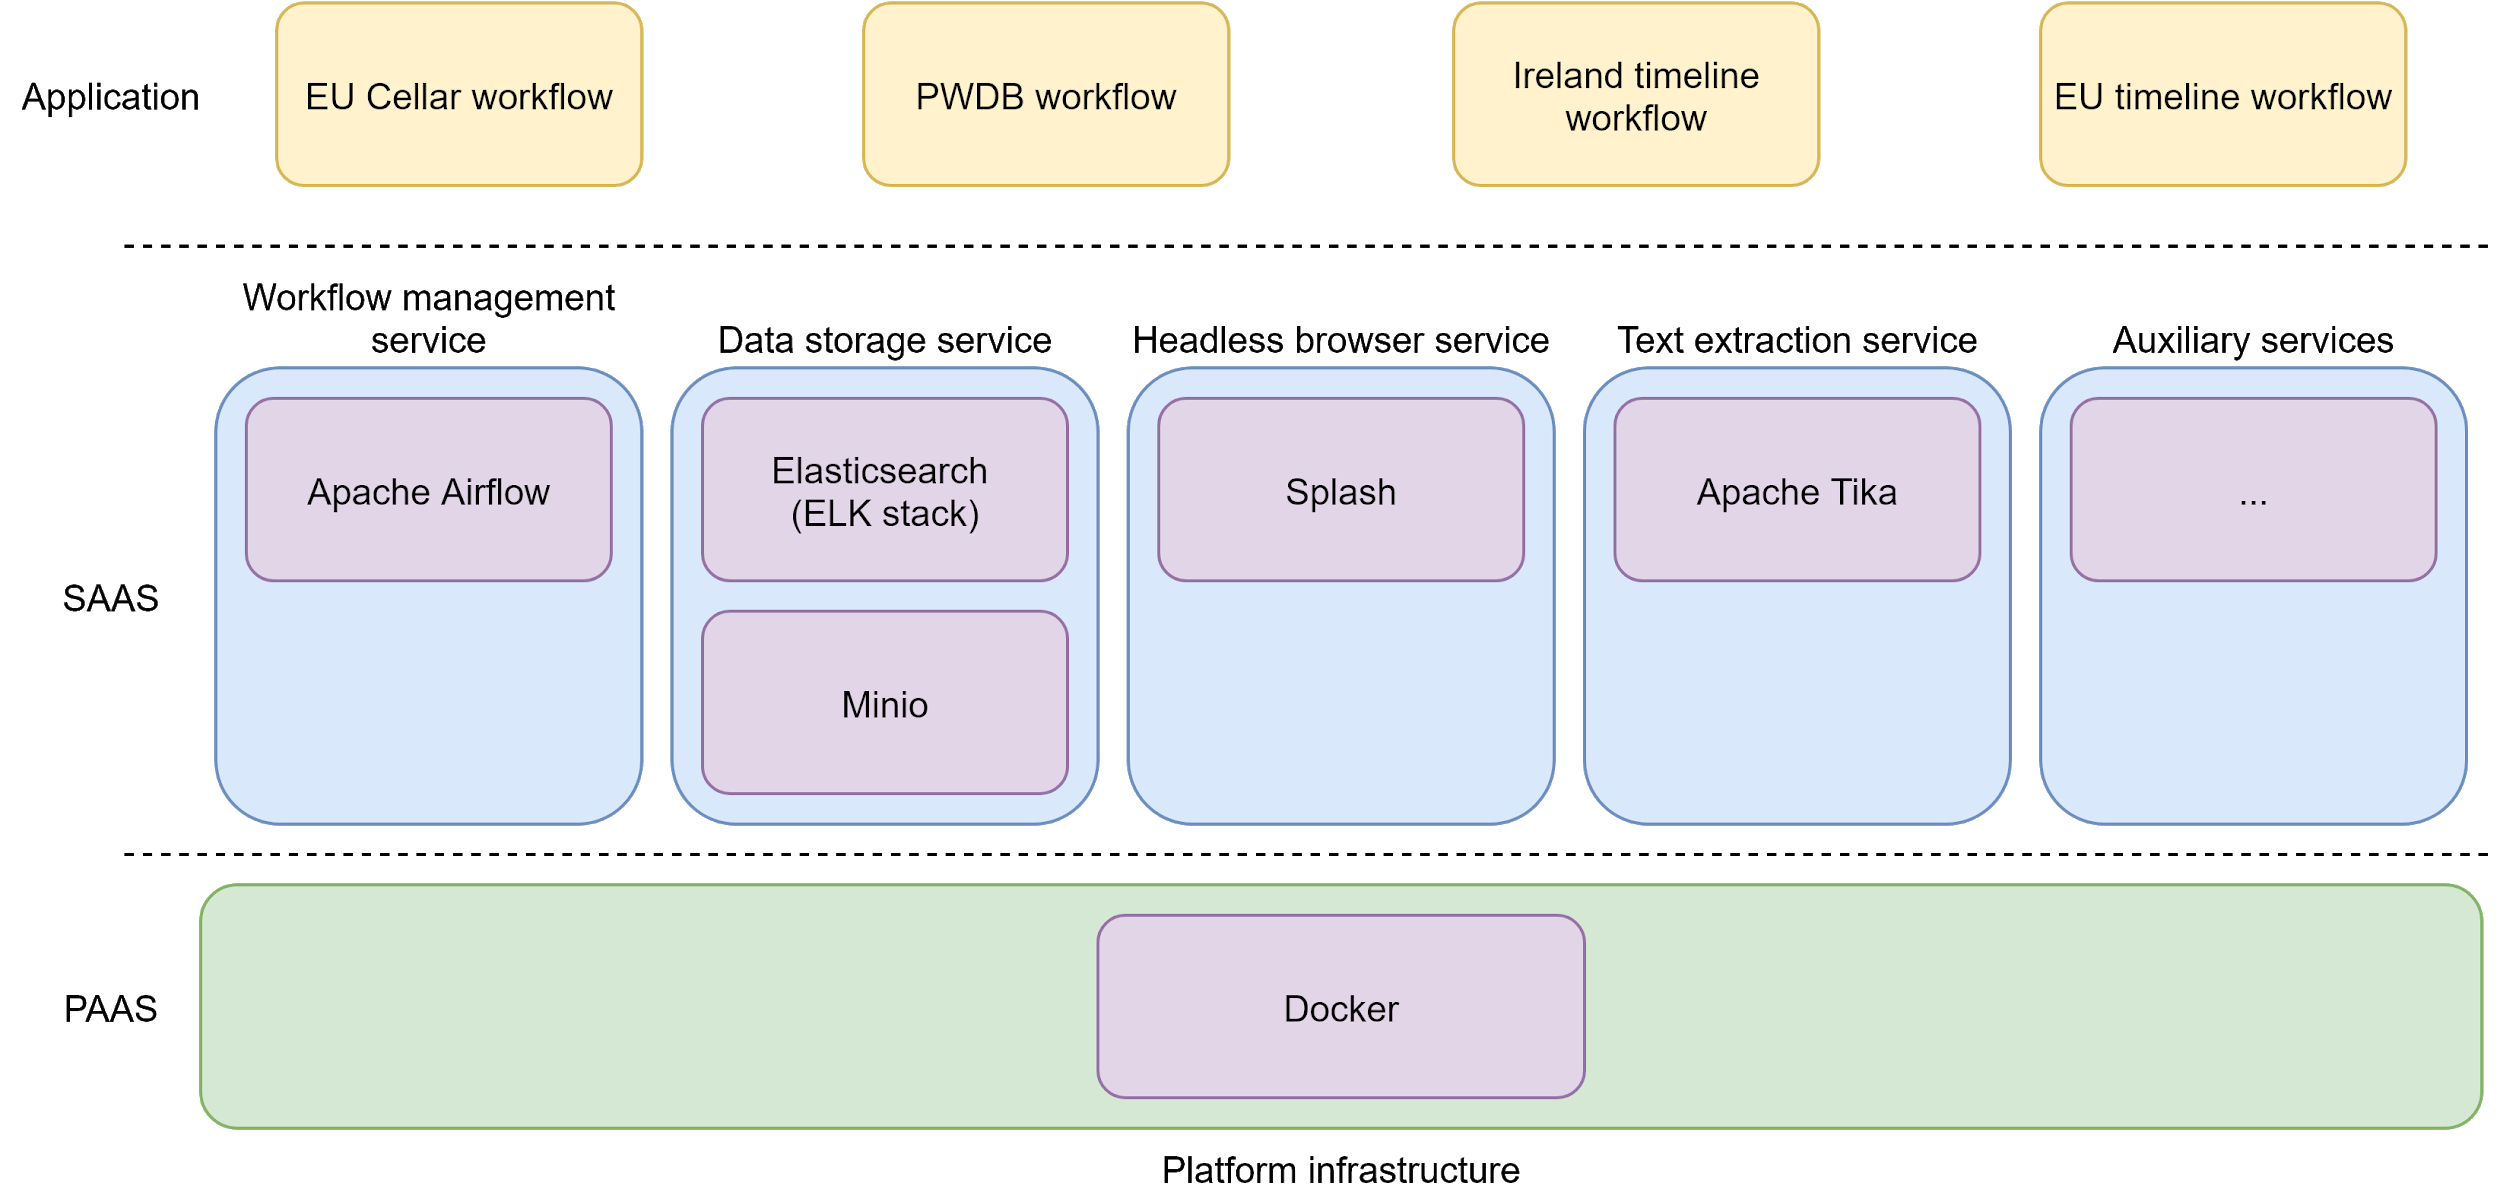
\includegraphics[width=\textwidth]{images/image3.png}
		\caption{Technology stack overview}
		\label{fig:Technology_stack_overview}
	\end{Center}
\end{figure}
%%%%%%%%%%%%%%%%%%%% Figure/Image No: 3 Ends here %%%%%%%%%%%%%%%%%%%%

The diagram in Figure \ref{fig:Technology_stack_overview} is split into three layers: \textit{Platform as a Service (PaaS) layer, Software as a Service (SaaS) layer, and Application layer}. 

\enlargethispage{2em}

At the bottom of the diagram is depicted the infrastructure layer. We have decided to operate based on a platform infrastructure because it abstracts away from the traditional physical servers and allows a deployment virtually in any environment: physical server, virtual machine, cloud. The chosen PaaS technology is Docker\footnote{Docker is a set of platform as a service (PaaS) products that use OS-level virtualization to deliver software in packages called containers. } for its popularity and relative simplicity over alternatives such as Kubernetes\footnote{Kubernetes is an open-source system for automating deployment, scaling, and management of containerized applications.}. 

In the middle of the diagram are depicted five larger blue round-cornered rectangles five. They represent classes of services we're employing in this project. These services are: \textit{workflow management system, data} \textit{storage service, headless browser service, text processing service, }and auxiliary services. We will explain below how each is used after we address the application layer workflow structure. 

In the top part of the diagram is depicted the application layer which contains four workflows, one for each dataset: \textit{EU Cellar workflow}, \textit{EU timeline workflow}, \textit{PWDB workflow}, and \textit{Ireland timeline workflow}. These workflows have a prototypical extract, transform, toad (ETL) structure\footnote{ In computing, extract, transform, load (ETL) is the general procedure of copying data from one or more sources into a destination system which represents the data differently from the source(s) or in a different context than the source(s). The ETL process became a popular concept in the 1970s and is often used in data warehousing. }. The generic ETL process implemented in our workflows is addressed in the next section.

\section{Workflow structure: how it works? }
\label{sec:how-it-works}

This section addresses the general structure of dataset creation workflow. Because it is a simple sequence of tasks, without any major bifurcations we call them pipelines as well. The prototypical pipeline we implement is depicted in Figure \ref{fig:Generic_ETL_process_for_dataset_creation} and can be conceptualised as a sequence of four steps: 

\begin{itemize}
	\item data\textit{ extraction} from the source and storage in the temporary object storage
	\item data \textit{structure transformation} in the temporary storage
	\item data \textit{content transformation} in the temporary storage

	\item final data\textit{ loading} into the document repository
\end{itemize}

The sources of data we employ in this project are: 

\begin{itemize}
	\item Cellar SPARQL endpoint\footnote{ \href{http://publications.europa.eu/webapi/rdf/sparql}{Cellar SPARQL endpoint} } where the EU legal documents are stored and disseminated. 
	\item Eurofound website\footnote{ \href{https://www.eurofound.europa.eu/data/covid-19-eu-policywatch}{Eurofound PWDB download page} } where the PWDB is published.
	\item EU action timeline page

	\item Ireland government press corner page
\end{itemize}

\begin{Center}
%%%%%%%%%%%%%%%%%%%% Figure/Image No: 4 starts here %%%%%%%%%%%%%%%%%%%%
\begin{figure}[h]
	\begin{Center}
		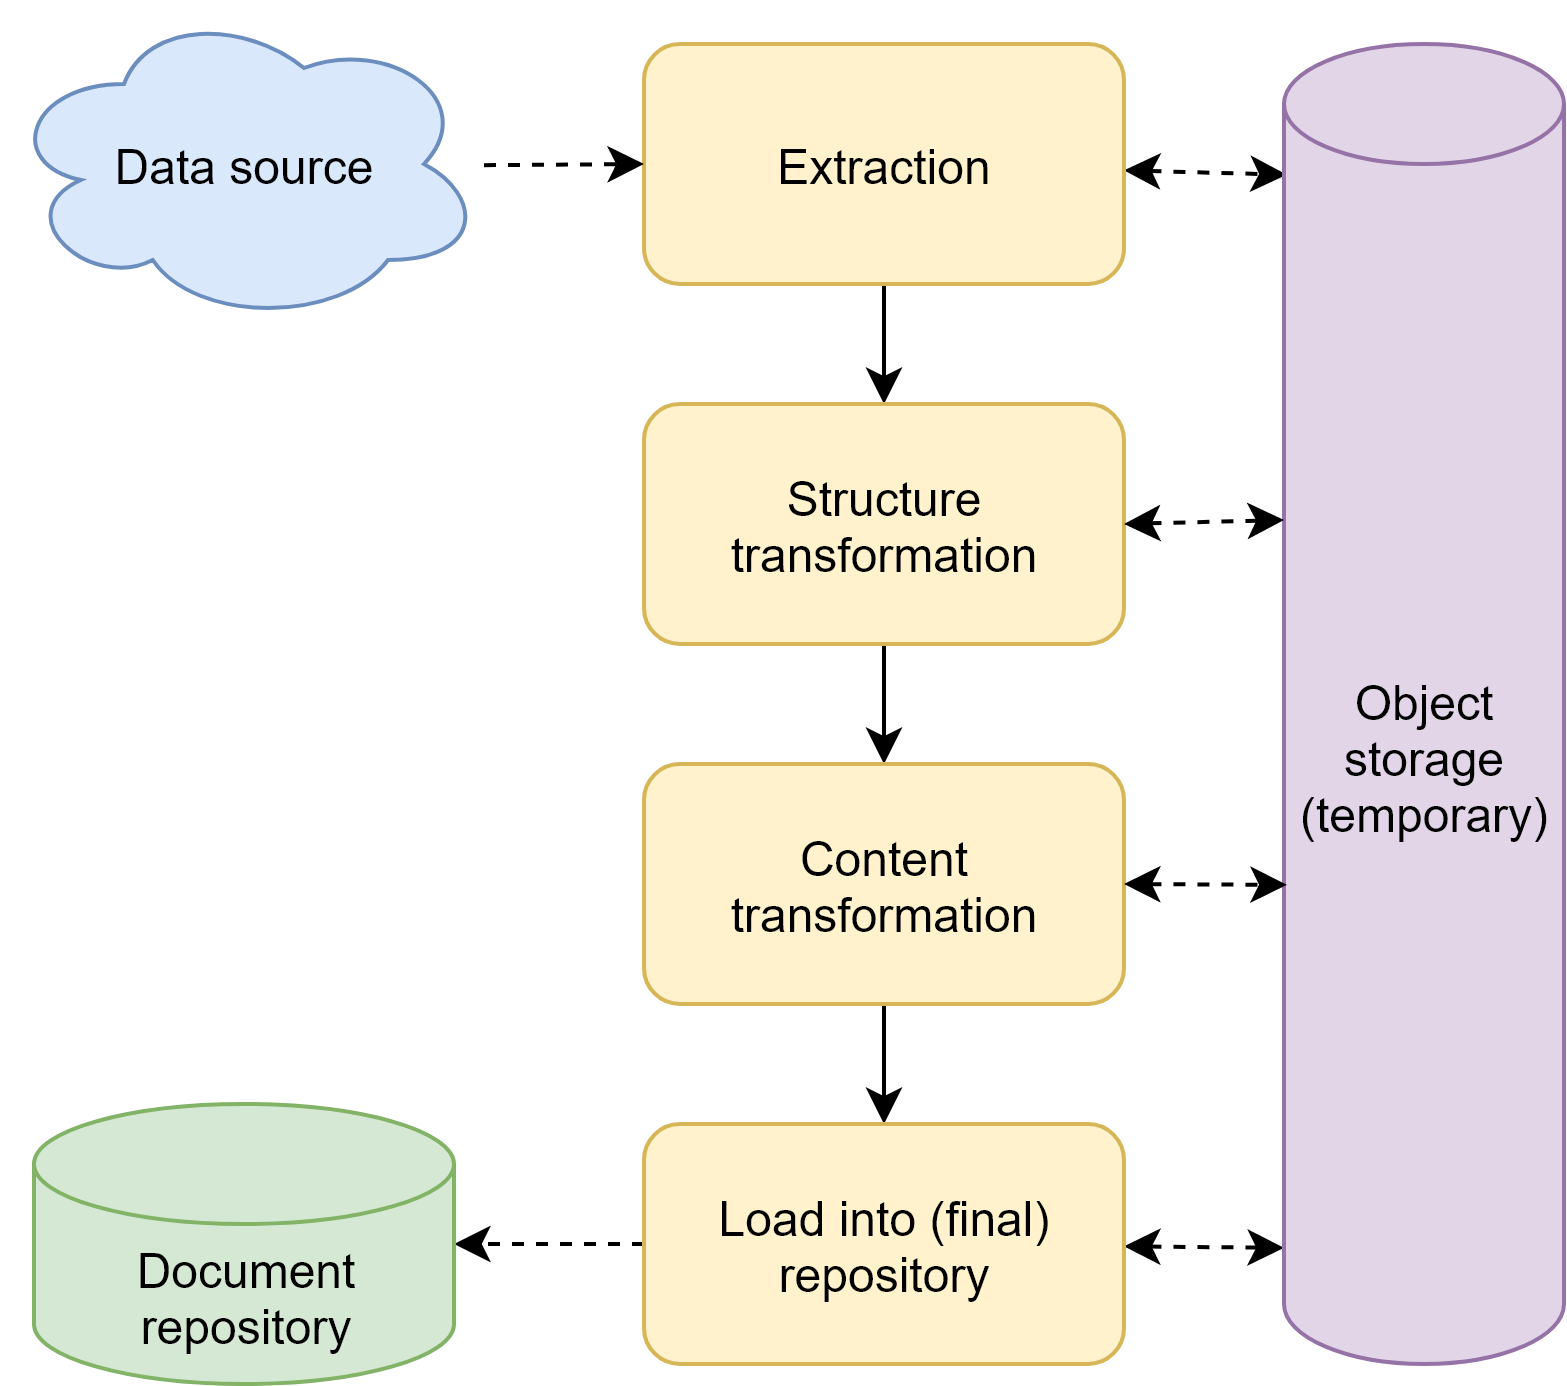
\includegraphics[width=4.24in,height=3.75in]{images/image5.png}
		\caption{Generic ETL process for dataset creation}
		\label{fig:Generic_ETL_process_for_dataset_creation}
	\end{Center}
\end{figure}
%%%%%%%%%%%%%%%%%%%% Figure/Image No: 4 Ends here %%%%%%%%%%%%%%%%%%%%
\end{Center}

\subsection{Extraction}

The process starts with \textit{extracting} the necessary data from the source and storing it in temporary object storage at our premises, making it available for further processing. Doing so enables us to process arbitrarily large amounts of data compared to the alternative of keeping the extracted data in memory, which is relatively limited on the traditional systems. 

Besides simple HTTP requests\footnote{ \href{https://en.wikipedia.org/wiki/Hypertext_Transfer_Protocol}{HTTP} is an application layer protocol for distributed, collaborative, hypermedia information systems. HTTP is the foundation of data communication for the World Wide Web. }, the extraction operations important to mention are the \textit{SPARQL querying} and \textit{Website crawling}. 

SPARQL\footnote{ \href{https://www.w3.org/TR/sparql11-query/}{SPARQL Protocol and RDF Query Language} } is a semantic query language able to retrieve and manipulate data stored in RDF\footnote{ \href{https://www.w3.org/TR/rdf11-concepts/}{Resource Description Framework}  } format. We query Cellar, the European semantic repository, for legal documents annotated with COVID-19 tag or related EuroVoc concepts. 

A \textit{Web crawler\footnote{ \href{https://en.wikipedia.org/wiki/Web_crawler}{Web crawler} }} sometimes called a \textit{spider} and often shortened to \textit{crawler}, is an Internet bot that systematically browses the World Wide Web, typically operated by search engines for the purpose of Web indexing. We developed two crawlers, using Scrapy library\footnote{ \href{https://en.wikipedia.org/wiki/Scrapy}{Scrapy}, a fast high-level web crawling $\&$  scraping framework for Python. }, first to fetch information from the EU action timeline website, and the second one from the Ireland government press corner. Scrapy is a free and open-source web-crawling framework written in Python. Originally designed for web scraping, it can also be used to extract data using APIs or as a general-purpose web crawler.

In the scraping process, often simple HTTP requests are not sufficient for performing full content extraction. Execution of custom JavaScript code is necessary to complete the page loading. For this purpose, headless browser services are typically implemented. They simulate the behaviour of a web browser but without having the interface of one. We employ Splash\footnote{ \href{https://splash.readthedocs.io/en/stable/}{Splash} javascript rendering service } to act as a headless browser. Splash is a javascript rendering service with an HTTP API. It's a lightweight browser with an HTTP API, implemented in Python 3. In combination with Scrapy, Splash allows us to crawl the two web sources successfully. 

One other aspect essential to mention here is that we employ an object storage service called Minio\footnote{ \href{https://min.io/}{MinIO} is an open source implementation of the Amazon S3 storage system.  } for the temporary persistence of the extracted data. MinIO is an Amazon S3 compatible server-side software storage stack. It can handle unstructured data such as photos, videos, log files, backups, and container images with the maximum supported object size of 5TB.

One may argue that such an object storage system is unnecessary as the created datasets, so far, are relatively small in size and can easily fit into the memory of most systems. However, this infrastructure, we intend to extend and use for the processing of much larger datasets exceeding the memory limits. That situation will inevitably invite the usage of such a persistence system, which we foresee and introduce upfront.

\subsection{Structure transformation}

Next, we proceed with \textit{structural transformation} to \textit{normalise} the data representation, simplify it, and increase its usability yet maintaining the maximally helpful structure. For convenience, we aim to represent the data in JSON format following the following system: \textit{an array of objects with a unique identifier and an arbitrary number of atomically typed attributes}. The structure is depicted using an example of prototypical JSON objects in Figure \ref{fig:Example_of_prototypical_JSON_objects_on_the_left_valid_and_on_the_right_an_invalid_structure}. 

The attributes may be of any atomic type, such as numbers, strings, dates, etc. or arrays of atomic types (as depicted on the left side of Figure \ref{fig:Example_of_prototypical_JSON_objects_on_the_left_valid_and_on_the_right_an_invalid_structure}), but not objects or arrays of objects (as depicted on the right side of Figure \ref{fig:Example_of_prototypical_JSON_objects_on_the_left_valid_and_on_the_right_an_invalid_structure}). We discourage, with some exceptions, using the embedded object structures. The reason for it is that the embedded objects are no longer easily accessible in the data frame structures (using the numpy\footnote{ Numpy is a library for the Python programming language, adding support for large, multi-dimensional arrays and matrices, along with a large collection of high-level mathematical functions to operate on these arrays. } or Pandas\footnote{ Pandas is a software library written for the Python programming language for data manipulation and analysis. } libraries). The data frames or other tabular representations are the de facto representation for machine learning and data science exercises, which we plan to undertake in the current project.

\begin{Center}
%%%%%%%%%%%%%%%%%%%% Figure/Image No: 5 starts here %%%%%%%%%%%%%%%%%%%%
\begin{figure}[H]
	\begin{Center}
		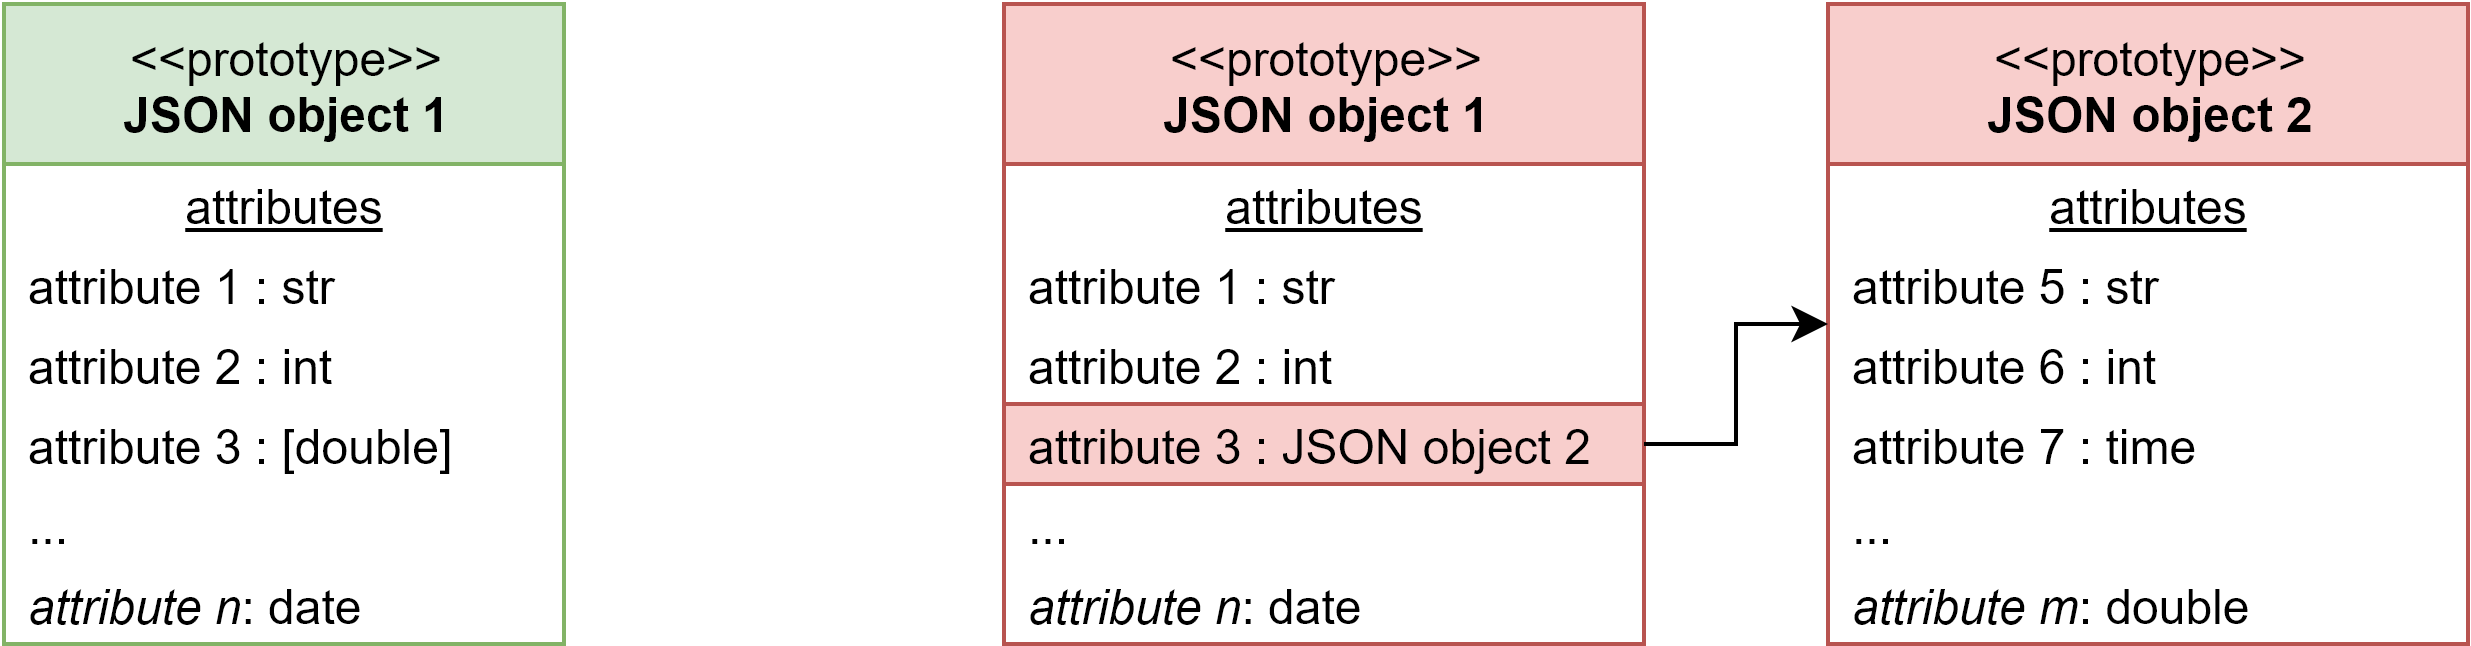
\includegraphics[width=\textwidth]{images/image1.png}
		\caption{Example of prototypical JSON objects, on the left valid and on the right an invalid structure}
		\label{fig:Example_of_prototypical_JSON_objects_on_the_left_valid_and_on_the_right_an_invalid_structure}
	\end{Center}
\end{figure}
%%%%%%%%%%%%%%%%%%%% Figure/Image No: 5 Ends here %%%%%%%%%%%%%%%%%%%%
\end{Center}

For consistency and programming language neutrality, we chose to employ JQ JSON processor\footnote{ ./jq is a lightweight and flexible command-line JSON processor }. The transformation rules are written in JQ language and tailor-made for each data source. As our implementation is entirely written in Python, we use the python library to execute these JQ transformation rules.

\subsection{Content transformation}

fter the data structure is \textit{normalised,} the content transformation generally consists of \textit{text extraction}, \textit{enrichment}, \textit{restructuring, aggregation,} and other operations. 

One peculiarity of this stage is that the initially extracted data contains links and references to other externally available resources. We have carefully analysed and decided to fetch the resources behind selected sets of links. Each dataset includes attributes with such links, which we access and inject the content as an additional attribute. This is what we call content enrichment: injecting extracted content into the dataset. 

The fetched content is in the majority of cases of unpredictable serialisation format, structure and language. Therefore, before it is injected into the dataset, we first \textit{reduce} it to simple texts, which is the foremost valuable data representation for the NLP tasks.

For the \textit{text extraction task,} we decided to use the Apache Tika\footnote{ Apache Tika is a toolkit that detects and extracts metadata and text from over a thousand different file types (such as HTML, PPT, XLS, and PDF). } toolkit. Apache Tika is a library that is used for document type detection and content extraction from various file formats. Internally, Tika uses existing different document parsers and document type detection techniques to detect and extract data. Tika is widely used while developing search engines to index the text contents of digital documents.

Some categorical data attributes are provided as items from a flat fine-grained classification. For practical reasons, it is helpful to reduce the classification scheme. This \textit{restructuring is possible to undergo} by \textit{aggregating} fine-grained categories in terms of more coarse-grained ones. One such example is the target group attribute from PWDB. There are 42 distinct values, which can be roughly categorised as belonging to three more prominent categories. We proceed to inject such aggregations as additional attributes to leverage exploratory data analysis in future stages of the project. 

\subsection{Loading into the repository}

After the structure and content of the data have been restructured, the data is loaded into a repository where it is indexed and made available for querying and full-text search. Because the current datasets are designed for NLP tasks, the full-text search capability is critical. It plays an essential role in the exploratory data analysis and possible data segmentation or partitioning for machine learning experiments. 

For this purpose, we decided to use the Elasticsearch search engine\footnote{ Elasticsearch is a search engine based on the Lucene library. It provides a distributed, multitenant-capable full-text search engine with an HTTP web interface and schema-free JSON documents. } to act as the document repository. It is a real-time distributed and analytic engine that helps in performing various kinds of search mechanisms. It can achieve fast search responses because, instead of searching the text directly, it searches an index instead. Additionally, it supports full-text search, which is completely based on documents instead of tables or schemas that are easier to write queries and manipulate with this textual data. Some of the strongest points of elastic search are:

\begin{itemize}
	\item Performing and combining various kinds of searches irrespective of their data type.
	\item Querying can retrieve data in any form required.
	\item Analyzing billions of records in a few seconds.
	\item Aggregating data enables us to explore trends and patterns.
\end{itemize}

When the datasets are loaded into the Elasticsearch, they are easily explorable using Kibana\footnote{ Kibana is a data visualization dashboard software for Elasticsearch. It provides visualization capabilities on top of the content indexed on an Elasticsearch cluster. } discovery and dashboard functionality. Kibana offers histograms, line graphs, pie charts, sunbursts, geospatial map displays, and other standard visualisation options and the opportunity to create unique visualisations. It also makes it possible for users to spot and analyse relationships or anomalies in the data. Furthermore, the datasets are available for use in machine learning experiments and exploratory data analysis. 

\section{Workflow management system}

The workflows mentioned above are deployed and executed in a workflow management system. Doing so drives automation and leads to increased control, transparency and trust in the execution results. It allows for close monitoring of each step, schedule executions, increased connectivity, eliminates manual tasks, reduces errors, retries on failure, and investigates causes and visualises the workflow, control panel, and other benefits. 

We have chosen Apache Airflow system\footnote{ Apache Airflow is an open-source workflow management platform. It started at Airbnb in October 2014 as a solution to manage the company's increasingly complex workflows. } due to its architectural choices, maturity, rich set of features, strong community, rich set of integrations and plugins, and because a system implemented in Python fits well our Python predominant technical stack. 

Airflow is a platform to programmatically author, schedule and monitor workflows. It is written in Python, and workflows are created via Python scripts, called DAGs (Directed Acyclic Graphs). An example DAG structure is depicted in Figure \ref{fig:Example_of_a_DAG_structure}. 

Airflow is designed under the principle of ``\textit{configuration as code}'' . While other ``\textit{configuration as code}''  workflow platforms exist using markup languages like XML, using Python allows developers to import libraries and classes to help them create their workflows.

\begin{Center}
%%%%%%%%%%%%%%%%%%%% Figure/Image No: 6 starts here %%%%%%%%%%%%%%%%%%%%
\begin{figure}[H]
	\begin{Center}
		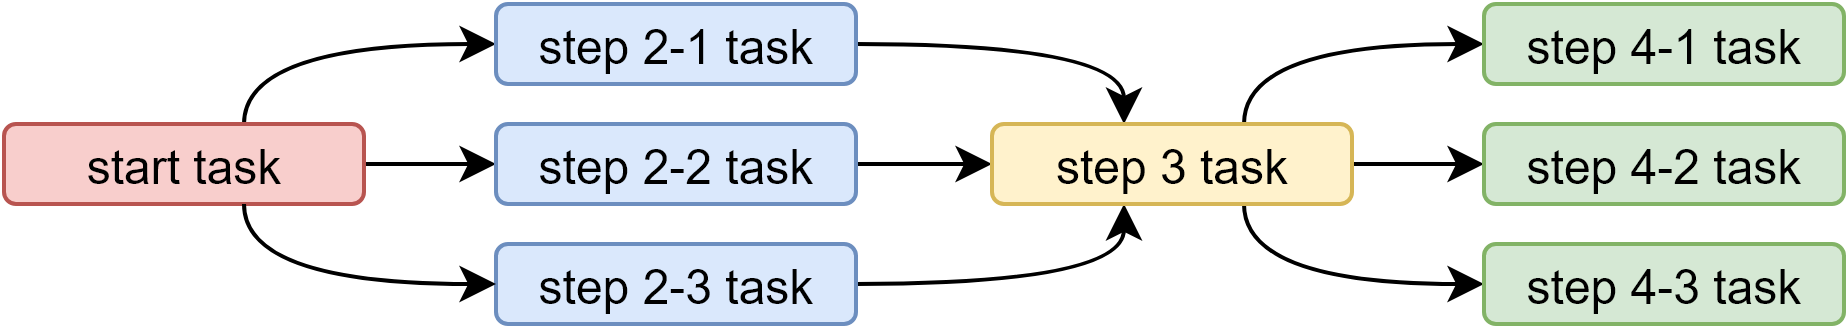
\includegraphics[width=\textwidth]{images/image2.png}
		\caption{Example of a DAG structure}
		\label{fig:Example_of_a_DAG_structure}
	\end{Center}
\end{figure}
%%%%%%%%%%%%%%%%%%%% Figure/Image No: 6 Ends here %%%%%%%%%%%%%%%%%%%%
\end{Center}

Airflow uses directed acyclic graphs (DAGs\footnote{ A DAG is a collection of all the tasks you want to run, organized in a way that reflects their relationships and dependencies. }) to manage workflow orchestration. Tasks and dependencies are defined in Python and then Airflow manages the scheduling and execution. DAGs can be run either on a defined schedule (e.g. hourly or daily) or based on external event triggers.

DAG, or directed acyclic graphs, are a collection of all of the tasks, units of work in the pipeline. The tasks are organised by their relationships and dependencies between each other. A directed acyclic graph implies that your pipeline can only move forwards, not backwards. A task can retry, but a task can't be rerun after it has completed and another task downstream has begun.

Using Airflow enables us to organise our pipelines as DAGs, develop project-specific functionality and incorporate it seamlessly into the workflow architecture to deploy and execute in a robust environment easily.

\section{Limitations and future work}

In the process of developing the current dataset, a number of limitations were set to the scope of this project. This section covers a non-exhaustive list of these limitations and how they may be addressed in future work.

Currently, the dataset is limited to the English language. In future work, the dataset can be expanded to cover member state measures individually. Doing so will inevitably lead to creating a multilingual dataset containing texts in 24 official European languages. This is mainly because the authorities publish the measures in that country's official language(s).

Using different text registers implies a disparate treatment of texts in the analysis and processing pipelines. Developing a mechanism to summarise a document to extract measure description from it, as, for example, would be necessary for large legal texts, would be of tremendous benefit for harmonisation of the dataset content across various sources. Addressing this in future work will yield an advantage for the exploratory data analysis and other machine learning exercises.

Another axis of homogenisation would be to bring all the texts to a common language, such as English, for example. To do so would necessitate translation services, which at the moment were not used. Having done so will decrease the linguistic fragmentation of the dataset, leading to a larger homogeneous corpus, which increases the statistical significance of the results produced based on this dataset.

\enlargethispage{2em}
